\pdfoutput=1
%% ****** Start of file apstemplate.tex ****** %
%%
%%
%% This file is part of the APS files in the REVTeX 4 distribution.
%% Version 4.1r of REVTeX, August 2010
%%
%%
%% Copyright (c) 2001, 2009, 2010 The American Physical Society.
%%
%% See the REVTeX 4 README file for restrictions and more information.
%%
%
% This is a template for producing manuscripts for use with REVTEX 4.0
% Copy this file to another name and then work on that file.
% That way, you always have this original template file to use.
%
% Group addresses by affiliation; use superscriptaddress for long
% author lists, or if there are many overlapping affiliations.
% For Phys. Rev. appearance, change preprint to twocolumn.
% Choose pra, prb, prc, prd, pre, prl, prstab, prstper, or rmp for journal
% Add 'draft' option to mark overfull boxes with black boxes
% Add 'showpacs' option to make PACS codes appear
% Add 'showkeys' option to make keywords appear
\documentclass[aps,prd,twocolumn,superscriptaddress,preprintnumbers,floatfix,nofootinbib]{revtex4-2}
%\documentclass[aps,prl,preprint,superscriptaddress]{revtex4-1}
%\documentclass[aps,prl,reprint,groupedaddress]{revtex4-1}

\usepackage{graphicx}
\usepackage{amsmath}
%\usepackage{mdwlist}
\usepackage[caption=false]{subfig}
\usepackage{siunitx}
\usepackage{placeins}
\usepackage{color}
\usepackage{standalone}
\usepackage{dcolumn}
\usepackage{tensor}
\usepackage{bm}
%\usepackage{MnSymbol}
\usepackage{microtype}
\usepackage{etoolbox}
\usepackage{amssymb}
\usepackage{mathrsfs}
\usepackage{accents}
\usepackage[normalem]{ulem}
\usepackage[dvipsnames]{xcolor}
\usepackage[colorlinks,urlcolor=NavyBlue,citecolor=NavyBlue,linkcolor=NavyBlue,pdfusetitle]{hyperref}
\usepackage[all]{hypcap}
\usepackage[inline]{enumitem}
\usepackage[utf8]{inputenc}
\usepackage{csquotes}
\usepackage{array}
\usepackage{booktabs}
%\usepackage[T1]{fontenc}
%\usepackage{lmodern}
\usepackage{wasysym}
\usepackage[nolist,nohyperlinks]{acronym}

\newcommand{\ts}{\textsuperscript}

\newcommand{\beq}{\begin{equation}}
\newcommand{\eeq}{\end{equation}}

\newcommand{\nn}{\nonumber}

\newcommand*{\eq}[1]{Eq.~\eqref{eq:#1}}
\newcommand*{\fig}[1]{Fig.~\ref{fig:#1}}
\newcommand*{\sect}[1]{Sec.~\ref{sec:#1}}

%% Try to control orphans, widows, and extra whitespace
%\widowpenalty=10000
%\clubpenalty=10000
%\raggedbottom
\interfootnotelinepenalty=3000

%% Enable/disable comments
\newtoggle{commentsoff}
\togglefalse{commentsoff}
%\toggletrue{commentsoff}

% Check for command-line option to turn comments off
% https://tex.stackexchange.com/questions/1492/passing-parameters-to-a-document
\ifdefined\nocomments
    \toggletrue{commentsoff}
\fi

\iftoggle{commentsoff}{
  \newcommand*{\mi}[1]{}
  \newcommand*{\comment}[1]{}
  \newcommand*{\suggest}[3]{#2}
  \newcommand*{\todo}[1]{}
  \newcommand*{\warn}[1]{}
  \newcommand*{\red}[1]{#1}
  \newcommand*{\blue}[1]{#1}
  \newcommand{\cn}{}
  \newcommand*{\commentmark}[1]{}
}{
  \newcommand*{\mi}[1]{{\color{magenta} [{\bf MAX}: #1]}}
  \newcommand*{\suggest}[3]{\textcolor{Purple}{\textbf{#3} \sout{#1} #2}}
  \newcommand*{\comment}[1]{{\color{blue} [{\bf NOTE}: #1]}}
  \newcommand*{\warn}[1]{{\color{red} [{\bf WARNING}: #1]}}
  \newcommand*{\todo}[1]{{\color{red} [{\bf TODO}: #1]}}
  \newcommand*{\red}[1]{{\color{purple} #1}}
  \newcommand*{\blue}[1]{{\color{blue} #1}}
  \newcommand{\cn}{\blue{\bf [cn]}}
}

\graphicspath{{./fig/}}

\newcommand{\dcc}{LIGO-PXXXXXXX}

% NOTATION MACROS
\newcommand{\infd}{\mathrm{d}}
\newcommand{\white}{\bar}

\begin{document}

% Use the \preprint command to place your local institutional report
% number in the upper righthand corner of the title page in preprint mode.
% Multiple \preprint commands are allowed.
% Use the 'preprintnumbers' class option to override journal defaults
% to display numbers if necessary
% \preprint{\dcc}

%Title of paper
\title{Parametrizing gravitational-wave polarizations}

\author{Maximiliano Isi}
\email[]{misi@flatironinstitute.org}
%\thanks{NHFP Einstein fellow}
%\homepage[]{Your web page}
%\thanks{}
%\altaffiliation{}
% \affiliation{
% LIGO Laboratory, Massachusetts Institute of Technology, Cambridge, Massachusetts 02139, USA
% }%
\affiliation{Center for Computational Astrophysics, Flatiron Institute, 162 5th Ave, New York, NY 10010}

% Because hyperref only gets the *last* author, we need to be explicit.
\hypersetup{pdfauthor={Isi}}



\date{\today}

\begin{abstract}
Amazing!
\end{abstract}

\maketitle

% \tableofcontents

\begin{acronym}
\acro{GW}{gravitational wave}
\acro{GR}{general relativity}
\acro{CBC}{compact-binary coalescence}
\end{acronym}

\section{Introduction}
\label{sec:intro}

\Acp{GW} come in two distinct polarization states, whose evolution encodes information about the dynamics of the source and the structure of \ac{GR}.
As for electromagnetic waves, these polarization states are only unambiguously defined up to rotations of the reference frame around the wave's direction of propagation.
When analyzing data from detectors like LIGO \cite{TheLIGOScientific:2014jea} and Virgo \cite{TheVirgo:2014hva}, it is necessary (or convenient) to parametrize these polarizations in different ways depending on the application.
For instance, searches for \acp{CBC} aim to relate the signal observed by different detectors to templates obtained from theory, and thus benefit from describing \ac{GW} polarizations in the same frame used to produce the predictions.
On the other hand, unmodeled (or semimodeled) analyses aim to reconstruct \acp{GW} without relying on specific input from theory, and must instead make an arbitrary choice in orienting the polarization frame.
Furthermore, lacking waveform templates, unmodeled analyses must also decide how to parametrize the \ac{GW} polarization state and its time evolution in a way sufficiently flexible to capture a range of morphologies but parsimonious enough to remain computationally tractable.
Analyses that focus on recovering signal power, without coherently modeling the phase evolution, may use yet different conventions.

Such ambiguities result in a variety of conventions for the definition and parametrization of \ac{GW} polarizations, both as described in the literature and as implemented in actual data analysis pipelines.
The result can not only be conceptually confusing to the uninitiated reader, but can also obfuscate comparisons across analyses with different conventions, or even difficult the interpretation the output of a given analysis.
Here I outline some useful alternatives and show how they are related.
It is important to understand the priors implied by the choice of parametrization through the corresponding Jacobians.

The goal of this note is twofold.
First, pedagogical, in reviewing different polarization conventions and their relation.
Second, technical, in providing explicit expressions for Jacobians relating different polarization parametrizations, ready for implementation in parameter estimation codes or similar applications.

This note is geared towards observers, or theorists interested in drawing connections to observation.
As such, it aims for concreteness, rather than comprehensiveness; it does not cover formal aspects of the frameworks connecting to the mathematical structure of general relativity and multipole expansions therein.
References are provided when such links are possible.

\section{Polarization primer}

\subsection{Linear basis}
\label{sec:linear}

In GR, there exist two propagating gravitational degrees of freedom, corresponding to two independent GW polarizations (e.g., \cite{Thorne1983,Thorne:1987af,Poisson2014,BT}).
At any given time, their local effect can be encoded in a driving matrix $h_{ij}$ representing the transverse-traceless part of the metric perturbation, also known as the \emph{gravitational-wave field}.
In a Cartesian frame with $z$-axis along the direction of propagation, we can write this matrix as
\beq \label{eq:hij}
(h_{ij}) = \begin{pmatrix}
h_+ & h_\times  & 0 \\
h_\times  & - h_+ & 0  \\
0 & 0 & 0
\end{pmatrix} ,
\eeq
where the plus ($+$) and cross ($\times$) polarization functions, $h_{+/\times}$, depend implicitly on the retarded time, $t - R/c$, in a way determined by the source dynamics and by the (luminosity) distance $R$ to the source.

\begin{figure}
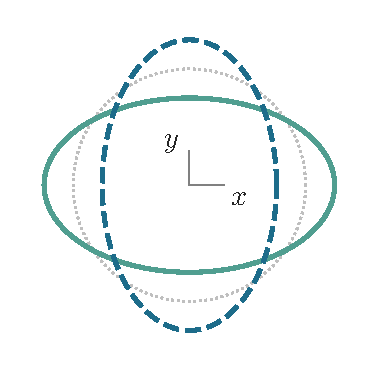
\includegraphics[width=0.4\columnwidth]{pol_ring_plus}
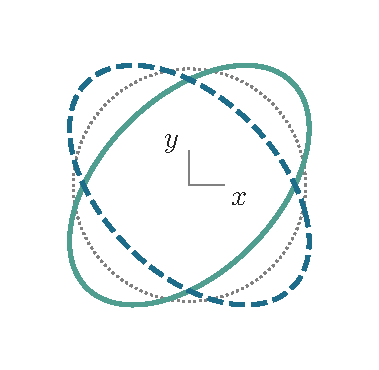
\includegraphics[width=0.4\columnwidth]{pol_ring_cross}
\caption{Effect of plus (left) and cross (right) polarizations on a small, freely falling ring of particles. The wave propagates in the $z$ direction, perpendicular to the page. The effect is illustrated half a period apart (solid vs dashed); the unperturbed ring is also shown for reference (thin dotted line).
}
\label{fig:rings}
\end{figure}

It can be useful to rewrite \eq{hij} as $h_{ij} = h_+ e^+_{ij} + h_\times e^\times_{ij}$, in terms of the $e^{+/\times}_{ij}$ polarization basis tensors given by
\begin{subequations} \label{eq:lin}
\begin{align}
e^+_{ij} &\equiv \hat{x}_i \hat{x}_j - \hat{x}_i \hat{x}_j \, ,\\
e^\times_{ij} &\equiv \hat{x}_i \hat{y}_j + \hat{x}_i \hat{y}_j\, ,
\end{align}
\end{subequations}
where $\hat{x}$ and $\hat{y}$ are arbitrary orthonormal vectors that, with $\hat{z}$, form a right-handed orthonormal basis; we will call this the \emph{wave frame}.
Since this frame is constructed to have $\hat{z}$ aligned with the wavevector $\vec{k}$ (i.e., $\hat{z} = \hat{k} \equiv \vec{k}/|k|$), the polarization tensors are implicit functions of the wave propagation direction $\hat{k}$, or, equivalently, the source sky location $\hat{n} = -\hat{k}$.
For a given $\hat{k}$, it is easy to check that these tensors are orthogonal such that $e^p_{ij} e^{p'ij}=2\delta^{pp'}$ for $p,p'$ in $\{+,\times\}$.
% Generic metric theories beyond GR generally predict up to four additional polarizations, which we briefly address in Sec.~\ref{sec:nongr}.

We will refer to plus and cross jointly as the \emph{linear} polarization basis.
Their physical interpretation is best illustrated by their instantaneous effect on a freely-falling ring of particles, as shown in Fig.~\ref{fig:rings}.
Other polarization bases can be constructed, as we will see below, but the linear polarizations are generally the most convenient for expressing measurements.

In the small-antenna limit, the signal induced by a passing GW on a given detector can be written as the projection
\beq \label{eq:h}
h(t) \equiv D^{ij} h_{ij} = F_+ h_+ + F_\times h_\times\, 
\eeq
with antenna patterns $F_{+/\times} \equiv D^{ij} e^{+/\times}_{ij}$ defined in terms of a detector tensor $D_{ij}$ that encodes the geometry of the measurement.
For a differential-arm detector like LIGO with arms pointing along unit vectors $\hat{X}$ and $\hat{Y}$, this is just $D_{ij} = (\hat{X}_i \hat{X}_j - \hat{Y}_i \hat{Y}_j)/2$.%
\footnote{These expressions are valid in the local Lorentz frame of the detector, so we can raise and lower indices with the flat metric.}
In this limit, the antenna patterns are thus purely geometric factors that encode the relative orientations of the detector and wave frames, as defined by $\{\hat{X},\, \hat{Y},\, \hat{Z}\}$ and $\{\hat{x},\, \hat{y},\, \hat{z}\}$ respectively.

% Equation \eqref{eq:hij} presumes a specific choice of wave frame orientation that defines the basis in which the $h_{ij}$ components are written.
% Although \eq{hij} requires that $\hat{z}$ be parallel to the (spatial) wave vector $\vec{k}$, there is no a priori restriction on the orientation of the $x$ and $y$ axes within the plane perpendicular to $\vec{k}$.
% %This freedom is usually encapsulated in the choice of an arbitrary \emph{polarization angle} $\psi$, defined with respect to some convenient reference (e.g., the celestial equator \cite{LALSuite:wave}).
% With some trigonometry, it is straightforward to show that a rotation of the frame by some angle $\Delta \psi$ around $z$ leaves the form of \eq{hij} unchanged after redefining
% \begin{subequations} \label{eq:htransf}
% \begin{align}
% h_+ &\rightarrow h_+' = h_+ \cos 2\Delta \psi - h_\times \sin 2\Delta\psi \, , \\
% h_\times &\rightarrow h_\times' = h_\times \cos 2\Delta \psi + h_+ \sin 2\Delta\psi \, .
% \end{align}
% \end{subequations}
% This reveals the fact that $h_+$ and $h_\times$ are nothing but the two components of a tensor field with spin-weight $|s|=2$, and the two polarizations are only defined up to an arbitrary rotation.
% (We return to this point in Sec.~\ref{sec:pol}.)

After fixing the frame orientation, any plane GW may be expressed in terms of the Fourier components of its polarization amplitudes as
\begin{align}
\label{eq:planewave}
h_{ij}(t,\vec{x}) &= \frac{1}{2\pi}\int_{-\infty}^{+\infty} \tilde{h}_{ij}(\omega, \hat{k})\, e^{i\omega \left(\frac{\hat{k}\cdot\vec{x}}{c}-t\right)} \infd \omega \\
&= \frac{1}{2\pi} \sum_{p=+,\times} \int_{-\infty}^{+\infty} \tilde{h}_p(\omega)\, e^p_{ij}(\hat{k})\, e^{i\omega \left(\frac{\hat{k}\cdot\vec{x}}{c}-t\right)} \infd \omega \nonumber
\end{align}
where the sum is over linear polarization states ($+,\times$) defined in some wave frame attached to the propagation direction $\hat{k}$,%
\footnote{More broadly, the strain value at any point in spacetime may be expressed with full generality as a superposition of these planewaves
% $h_{ij}(t,\vec{x}) = \int_{\mathcal{S}^2} \int_{-\infty}^{+\infty} \tilde{h}_p(\omega, \hat{k})\, e^p_{ij}(\hat{k})
% \exp\left[{i\omega \left(\hat{k}\cdot\vec{x}/c-t\right)}\right] \infd \omega \infd \hat{k}$
by integrating over all directions of propagation.}
and we obtained the second line using the fact that the $e^{+/\times}_{ij}$ are real valued.
Equation \eqref{eq:planewave} implicitly defines the complex-valued Fourier polarization functions $\tilde{h}_p(\omega)$ to correspond to the time-domain polarizations at the spatial origin, $h_p(t) \equiv h_p(t, \vec{x}=0)$, by
\beq \label{eq:ft}
\tilde{h}_p(\omega) \equiv \int_{-\infty}^{+\infty} h_p(t)\, e^{i\omega t} \infd t \, ,
\eeq
establishing our convention for the Fourier transform.

Since $h_{ij}$ is real valued, the Fourier strain must  satisfy the complex-conjugate symmetry $\tilde{h}_{ij}(-\omega, \hat{k}) = \tilde{h}_{ij}^*(\omega,\hat{k})$, where the asterisk indicates complex conjugation.
For the linear polarizations, this reduces to
\beq \label{eq:sym_linear}
\tilde{h}_{+/\times}(\omega) = \tilde{h}_{+/\times}^*(-\omega)\, ,
\eeq
because the linear basis tensors are themselves real valued.
As usual, then, the positive and negative frequencies must be considered as inseparable contributions to a single Fourier mode.
The existence of this symmetry reveals a redundancy in the description that we can exploit to write Eq.~\eqref{eq:planewave} more concisely.

\begin{figure*}
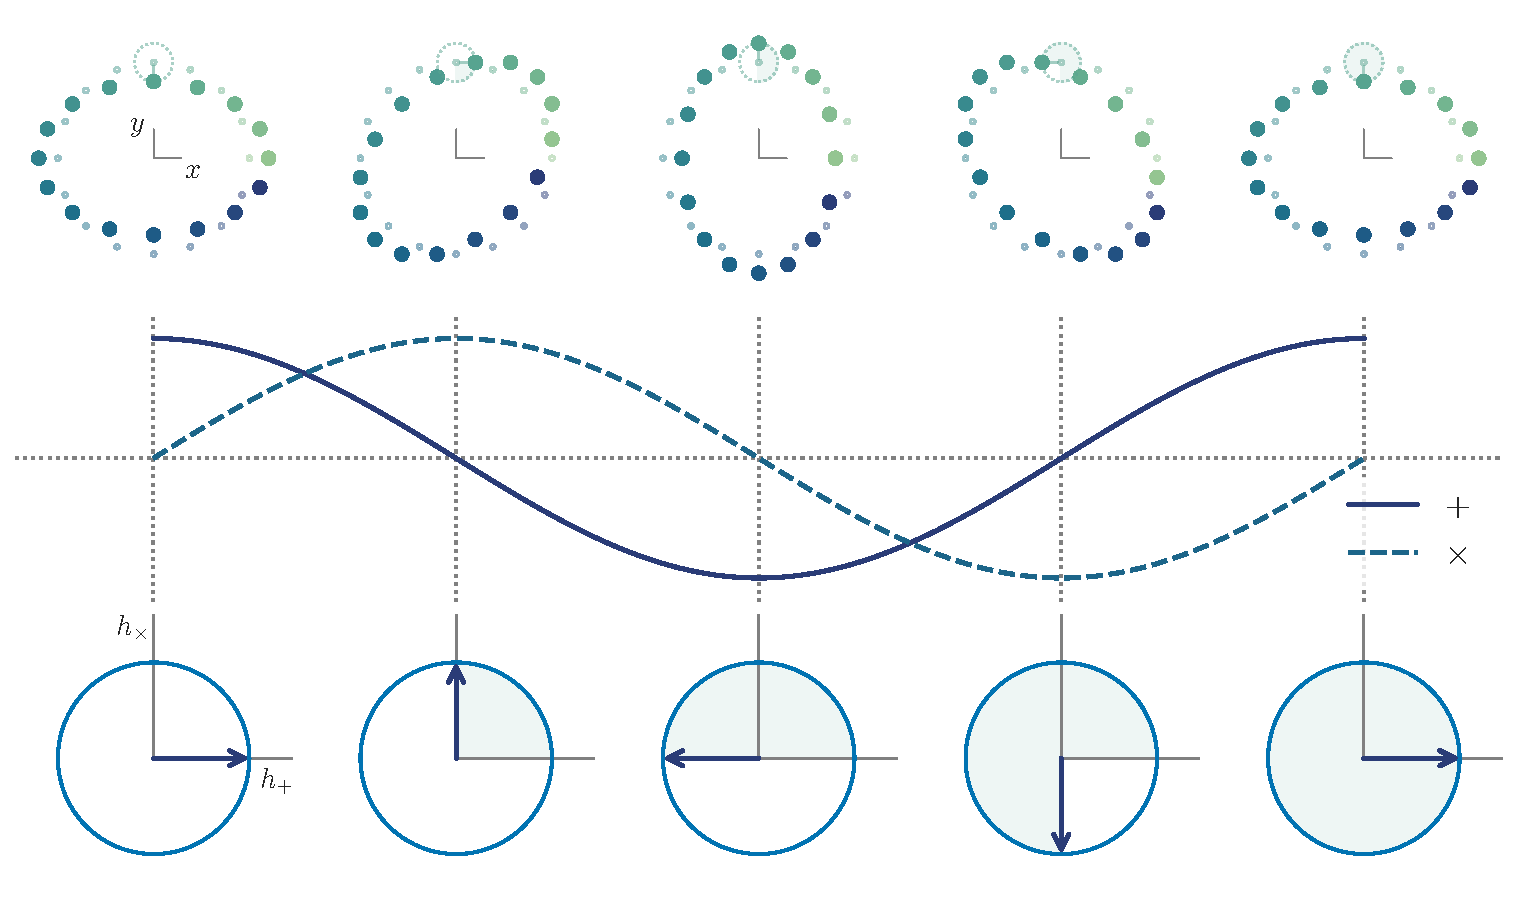
\includegraphics[width=0.8\textwidth]{pol_diagram_circ}
\caption{A right-handed, circularly polarized GW as a function of time (left to right) over a period. \emph{Top:} as the wave propagates out of the page, it deforms a freely falling ring of particles (colored dots) into an ellipsoidal pattern, which rotates counterclockwise with time; each individual particle is pushed in a circle around its original location, i.e., the location it would have had in absence of the wave (small empty circles).
\emph{Middle:} amplitudes of the plus (solid) and cross (dashed) linear polarizations making up the wave as a function of time; the plus polarization is $\pi/2$ radians ahead of the cross polarization.
\emph{Bottom:} representation of the polarization state as a Jones vector in the $+$ and $\times$ space; the phasor rotates counterclockwise in a circle.
Reversing the direction of time by reading this diagram right-to-left gives the effect of a left-handed circularly polarized wave.
}
\label{fig:pol_diagram_circ}
\end{figure*}

\subsection{Circular basis}

First, instead of the linear plus and cross polarizations above, we could equivalently work with the associated \emph{circular} right-handed (R) and left-handed (L) modes.
%, which are eigenstates of the helicity operator.
These are defined in the Fourier domain by the complex-valued basis tensors
\beq \label{eq:circ}
e^{R/L}_{ij} \equiv \frac{1}{\sqrt{2}} \left(e^+_{ij} \pm i e^\times_{ij} \right) ,
\eeq
with the plus (minus) sign corresponding to R (L).
These tensors are also orthogonal and normalized similarly to $e^{+/\times}_{ij}$ such that $(e^{p'ij})^* e^p_{ij} = 2 \delta^{pp'}$ for $p,p'$ in $\{R,L\}$.

To understand the physical significance of the circular polarizations,
% consider an individual Fourier mode of frequency $\omega>0$ propagating in the positive-$z$ direction,
% \beq
% h_{ij}(t,z; \omega) = \Re \left\{ \tilde{H}_{ij} \exp[ i \omega (z/c - \omega t)]\right\},
% \eeq
% for some time and location independent (and complex-valued) amplitude tensor $\tilde{H}_{ij}$.
consider a purely R-polarized monochromatic mode $h^R_{ij}$ with frequency $\omega > 0$, unit amplitude and zero phase offset; at the spatial origin ($\vec{x}=0$), the time-domain strain from such a mode will be given by
\begin{align} \label{eq:circ_example}
h_{ij}^R(t;\omega) &= \Re \left[ e^R_{ij}\, \exp(-i\omega t) \right] \nonumber\\
%&= \frac{1}{\sqrt{2}} \Re \left[\left(e^+_{ij} + i e^\times_{ij}\right) \exp(-i\omega t) \right] \nonumber\\
&= \frac{1}{\sqrt{2}} \left( e^+_{ij} \cos \omega t + e^\times_{ij} \sin \omega t \right) ,
\end{align}
using the definition from Eq.~\eqref{eq:circ}.
In the 2D Cartesian space defined by the linear polarization amplitudes, i.e. $\left(h_+, h_\times\right)$, this defines a circle, around which the \emph{phasor} encoding the state of the wave rotates counterclockwise (for $\omega > 0$).
This means that, at any given time, the wave will have a unit total amplitude (i.e., $h^2_+ + h^2_\times=1$) and the cross polarization will \emph{lag behind} the plus polarization by $\pi/2$ radians in phase.
%
Consequently, a purely R-polarized wave will deform a ring of freely-falling particles into an elliptical pattern that is seen to rotate counter-clockwise when looking towards the source (Fig.~\ref{fig:pol_diagram_circ}), i.e., it follows the right-hand rule relative to the direction of propagation (pointing away from the source).
The opposite will be true for purely L-polarized waves, which will result in a clockwise-rotating ellipse.
%\footnote{If we let $\omega < 0$ then the roles of R and L would flip, indicating these states are invariant under parity-time transformations.}
This assignment of the ``right'' and ``left'' labels is known as the ``source based'' handedness convention.

The orthogonality and completeness of the tensors in Eq.~\eqref{eq:circ} mean that we can rewrite Eq.~\eqref{eq:planewave} in terms of the circular polarizations without loss of generality as the sum
\beq \label{eq:planewave_circ}
h_{ij}(t,\vec{x}) 
= \frac{1}{2\pi} \sum_{p=R,L} \int_{-\infty}^{+\infty} \tilde{h}_p(\omega)\, e^p_{ij}(\hat{k})\, e^{i\omega \left(\frac{\hat{k}\cdot\vec{x}}{c}-t\right)} \infd \omega \, ,
\eeq
where $\tilde{h}_{R/L}$ and $e^{R/L}_{ij}$ have replaced their $+/\times$ counterparts.
As is straightforward to show from Eq.~\eqref{eq:circ}, the circular and linear polarization Fourier amplitudes are related by
\begin{align} \label{eq:circ_amps}
\tilde{h}_{R/L} = \frac{1}{\sqrt{2}} \left(\tilde{h}_+ \mp i\tilde{h}_\times \right) ,
\end{align}
with the minus (plus) sign for R (L).
Based on this, the complex-conjugate condition of Eq.~\eqref{eq:sym_linear} implies that
\beq \label{eq:sym_circular}
\tilde{h}_R(\omega) = \tilde{h}_L^*(-\omega) \, ,
\eeq
which again manifests the redundancy in Eq.~\eqref{eq:planewave_circ}, as in Eq.~\eqref{eq:planewave}.
It also reveals that R and L switch roles for $\omega \to - \omega$, as we anticipated below Eq.~\eqref{eq:circ_example}, indicating that these states are invariant under parity-time reversals.


\subsection{Elliptical basis}
\label{sec:ellip}

%\subsubsection{Complex strain}

Next, it is convenient to encode the two linear GW polarizations as quadratures of a single complex-valued scalar field, 
\beq
H(t) \equiv h_+ - i h_\times,
\eeq
in the time domain.
This complex number provides an alternative representation of the $\left(h_+, h_\times\right)$ phasor introduced in the previous section (see bottom panel of Fig.~\ref{fig:pol_diagram_circ}).
If this quantity, the \emph{complex strain}, is purely real (imaginary), then the wave is purely plus (cross) polarized.
In those same terms, a unit-amplitude circularly-polarized mode like the one in \eq{circ_example} can be expressed simply as $H(t)  = \exp(\mp i \omega t)/\sqrt{2}$, with the minus (plus) sign in the exponent corresponding to R (L) for $\omega > 0$.%
\footnote{The choice of sign in the definition of the complex strain as $h_+ - ih_\times$ matches the convention of the Fourier transform in Eq.~\eqref{eq:ft} in order to make it so that $\exp(-i|\omega| t)$ encodes a right-handed mode as defined in the source-based convention.}

Using this fact, an economic way of expressing the information in Eq.~\eqref{eq:planewave} for any given direction of propagation $\hat{k}$ is to write the time-domain complex strain at the spatial origin ($\vec{x}=0$) as a Fourier integral of the form
\begin{align} \label{eq:hcomp_fd}
H(t) = \frac{1}{2\pi} \int_{-\infty}^{+\infty} \tilde{H}(\omega)\, e^{-i \omega t} \,\infd \omega \, ,
\end{align}
where the complex-valued Fourier amplitudes are defined by $\tilde{H}(\omega) \equiv \int (h_+ - i h_\times) \exp(i\omega t)\, \infd t = \tilde{h}_+(\omega) - i \tilde{h}_\times(\omega)$, following our Fourier transform convention in Eq.~\eqref{eq:ft}.
Unlike in Eq.~\eqref{eq:planewave}, it is clear that these Fourier amplitudes will not generally satisfy the symmetry $\tilde{H}(-\omega) = \tilde{H}^*(\omega)$, since the quantity on the left hand side of Eq.~\eqref{eq:hcomp_fd} is not real-valued unless the wave is fully plus-polarized.

In fact, given the interpretation of $\exp(\pm i \omega t)$ discussed above, the positive (negative) frequency Fourier amplitudes in Eq.~\eqref{eq:hcomp_fd} must encode contributions from the R-polarized (L-polarized) portion of the waveform.
This becomes obvious if we note that, by Eq.~\eqref{eq:circ_amps} and the definition of $\tilde{H}$, it must be the case that $\tilde{H}(\omega) = \sqrt{2}\, \tilde{h}_R (\omega) = \sqrt{2} \tilde{h}_L^*(-\omega)$, the last equality being due to Eq.~\eqref{eq:sym_circular}.
We can leverage this to rewrite Eq.~\eqref{eq:hcomp_fd} as an integral restricted to positive frequencies,
\begin{equation} \label{eq:hcomp_fd_rl}
H(t) = \frac{1}{\sqrt{2\pi^2}} \int_{0}^{\infty} \left[ \tilde{h}_R(\omega)\, e^{-i \omega t} + \tilde{h}_L^*(\omega)\, e^{i \omega t}\right] \infd \omega \, .
\end{equation}
This expression carries the same information as Eq.~\eqref{eq:planewave} without any redundancies.

\begin{figure}
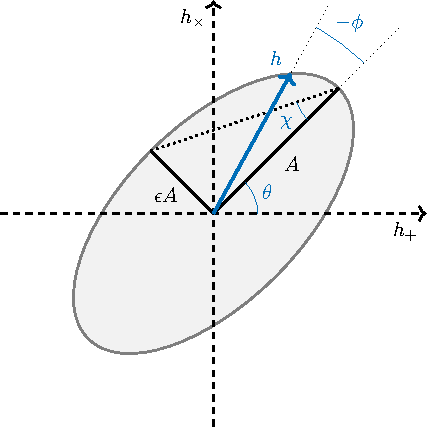
\includegraphics[width=0.65\columnwidth]{diagram_ellipse.pdf}
\caption{Polarization ellipse. Following \eq{hcomp_ellip}, at any given time, the phasor (blue arrow) of an elliptically polarized signal lies on an ellipse with some maximum amplitude $A$ and ellipticity $\epsilon$, with semimajor axis tilted by an angle $\theta$ with respect to the plus-polarization axis (abscissa); a second angle, $\phi$, determines the initial location of the phasor within the ellipse.
The shape of the ellipse can also be parametrized in terms of the angle $\chi \equiv \arctan \epsilon$.
The domain for these parameters is $A \geq 0$, $-1 \leq \epsilon \leq 1$, $-\pi/4 \leq \chi \leq \pi/4$, $0 \leq \theta < \pi$ and $0 \leq \phi < \pi$ (or, equivalently, $-\pi/2 \leq \theta < \pi/2$ and $-\pi/2 \leq \phi < \pi/2$).
}
\label{fig:ellipse}
\end{figure}

Equation \eqref{eq:hcomp_fd_rl} lends itself to a straightforward physical interpretation.
Any plane GW, with arbitrary time evolution and polarization state (including unpolarized states), can be expressed as a superposition of fully-polarized Fourier modes;
each such monochromatic mode of frequency $|\omega|$ is made up of two counterrotating circularly-polarized contributions (R and L, the two summands) that add up to a single elliptically polarized mode.
Such elliptical, or \emph{fully-polarized}, modes are thus of fundamental importance; we discuss their properties in detail below, beginning with modes of a definite frequency as they appear in \eq{hcomp_fd_rl}.

\section{Elliptical modes}
\label{sec:ellip}

\subsection{Monochromatic modes}
\label{sec:ellip:mono}

\subsubsection{Morphology}

Elliptical GWs define an ellipse in the $\left(h_+, h_\times\right)$ phasor space (Fig.~\ref{fig:ellipse}).
We can see this explicitly for the Fourier modes in Eq.~\eqref{eq:hcomp_fd_rl} above by considering a monochromatic signal given by $\tilde{h}_{R/L}(\omega) = \pi\, \delta(\omega-\omega_0)\, C_{R/L} $,%
\footnote{The prefactor can be motivated by noting that $\tilde{h}_{R/L}(\omega) = 2\pi \delta(\omega - \omega_0) C_{R/L}/2 = \delta(f - f_0) C_{R/L} / 2$ implies that $C_{R/L}/2$ are amplitude densities with respect to the frequency $f \equiv \omega/2\pi$; the additional factor of $1/2$ normalizes the signal power such that $h_+^2 + h_\times^2 = 1$ for $|C_R|=1, |C_L|=0$ or $|C_R|=0, |C_L|=1$.}
isolating a single Fourier mode of frequency $\omega_0 >0$ and complex-valued amplitudes $\pi\, C_{R/L}$.
The result of the Fourier integral for $H(t) \equiv h_+ - i h_\times$ is then (relabeling $\omega_0 \to \omega$ after integration)
\begin{align} \label{eq:ellip_circ}
H(t) =\frac{1}{\sqrt{2}} \left( C_R\, e^{-i \omega t} + C^*_L\, e^{i\omega t}\right)\, ,
\end{align}
for complex amplitudes $C_{R/L} \equiv A_{R/L} \exp(i\phi_{R/L})$, where $A_{R/L}$ and $\phi_{R/L}$ are real.
Without loss of generality, the above expression can be refactored into
\begin{align}
H(t) = \frac{1}{2}A\hspace{-2pt}\left[ \left(1+\epsilon\right) e^{-i (\omega t - \phi_R)} + \left(1-\epsilon\right) e^{i (\omega t - \phi_L)} \right]\hspace{-3pt} .
\end{align}
In this expression, 
$A \equiv (A_R + A_L)/ \sqrt{2} \geq 0$ is the peak amplitude of the mode, and $\epsilon = (A_R - A_L)/(A_R + A_L)$ is its ellipticity, with $-1 \leq \epsilon \leq +1$ by construction.
With some trigonometry, it is easy to show that this corresponds to linear polarization quadratures given by
\begin{subequations} \label{eq:hcomp_ellip}
\beq
h_+ = A \left[\cos \theta \cos(\omega t - \phi) - \epsilon \sin \theta \sin(\omega t - \phi)\right] ,
\eeq
\beq
h_\times = A \left[\sin \theta \cos(\omega t - \phi) + \epsilon \cos \theta \sin(\omega t - \phi)\right] ,
\eeq
\end{subequations}
with $\phi \equiv (\phi_L + \phi_R)/2$ and $\theta \equiv (\phi_L - \phi_R)/2$. 
In the $\left(h_+,h_\times\right)$ plane, this defines an ellipse with semimajor axis $A$ and semiminor axis $\epsilon A$, oriented as to subtend an angle $\theta$ between the semimajor axis and the $h_+$ axis, and with an initial location around the ellipse given by $-\phi$ (Fig.~\ref{fig:ellipse}).
The total power in this mode is given by the square of the \emph{intensity amplitude}, which we define as $\hat{A} \equiv \sqrt{A_R^2 + A_L^2} = A \sqrt{1 + \epsilon^2}$.

Equation \eqref{eq:hcomp_ellip} encapsulates all possible morphologies of a monochromatic, fully polarized wave.\footnote{We use ``elliptical'' generically to also encompass circular and linear polarizations as special cases; in this sense, ``elliptical'' and ``fully polarized'' are synonyms.}
As special cases, $\epsilon = +1$ ($\epsilon = -1$) encodes an R (L) circularly-polarized wave, while $\epsilon =0$ encodes a $+$ ($\times$) linearly-polarized wave if $\theta = 0,\pi$ ($\theta = \pm \pi/2$);
an example in between, with $\epsilon=1/2$ and $\theta = \pi/2$, is illustrated in Fig.~\ref{fig:pol_diagram_ellip} (compare to Fig.~\ref{fig:pol_diagram_circ}, where $\epsilon=1$).
Each Fourier component in Eq.~\eqref{eq:hcomp_fd_rl} is a fully polarized mode of this kind, with ellipticity determined by the relative magnitudes of $\tilde{h}_{R/L}(\omega)$, and ellipse orientation determined by the difference in their Fourier phases, through $\theta = (\arg \tilde{h}_L - \arg \tilde{h}_R)/2$.

\begin{figure*}
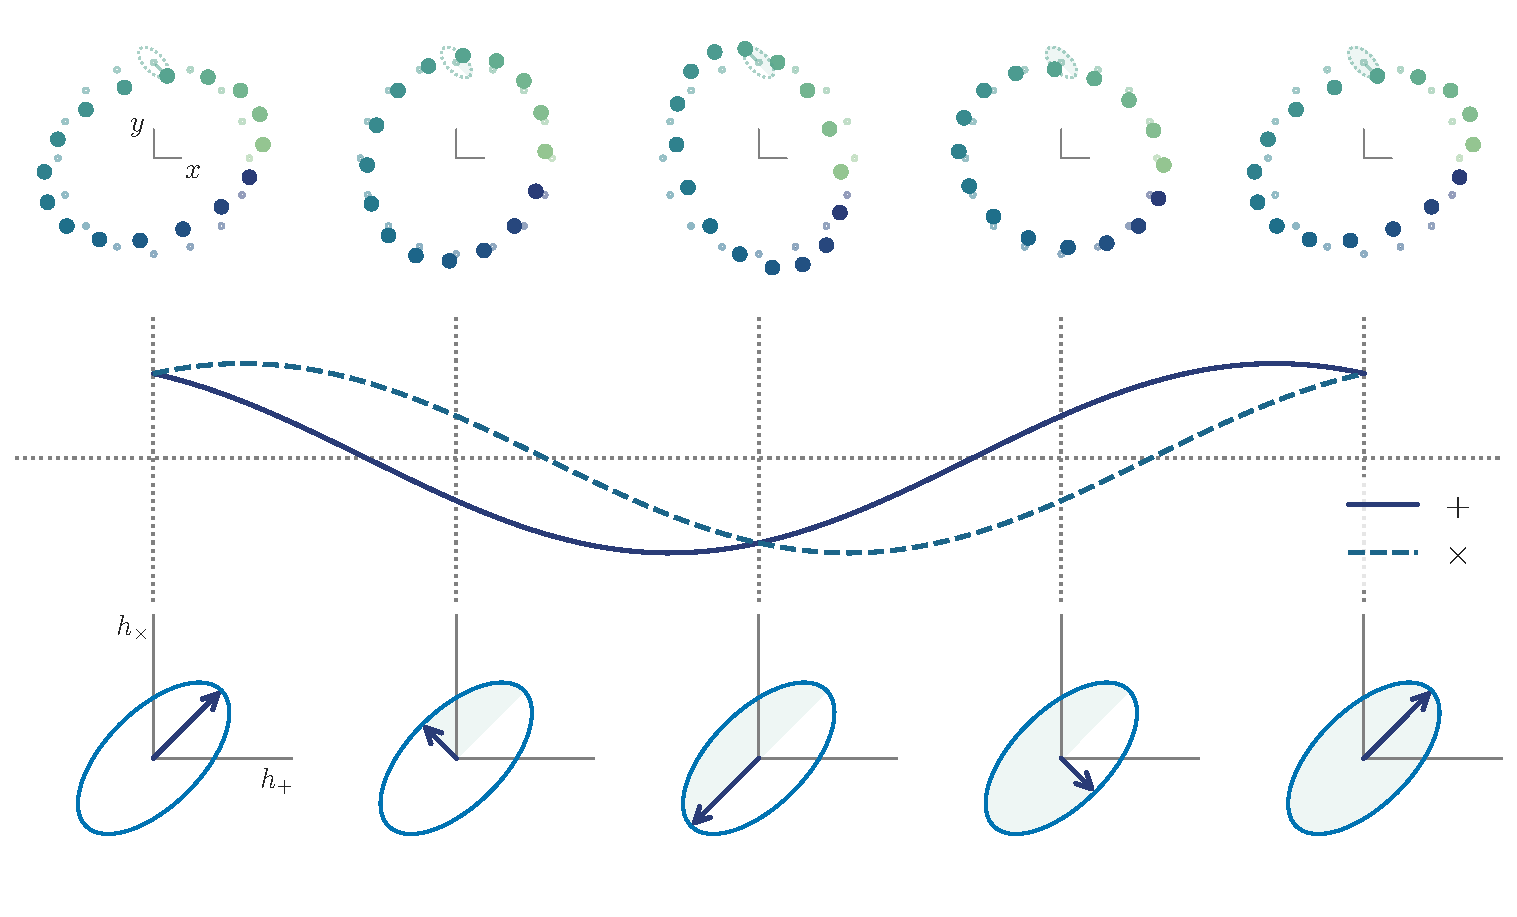
\includegraphics[width=0.8\textwidth]{pol_diagram_ellip}
%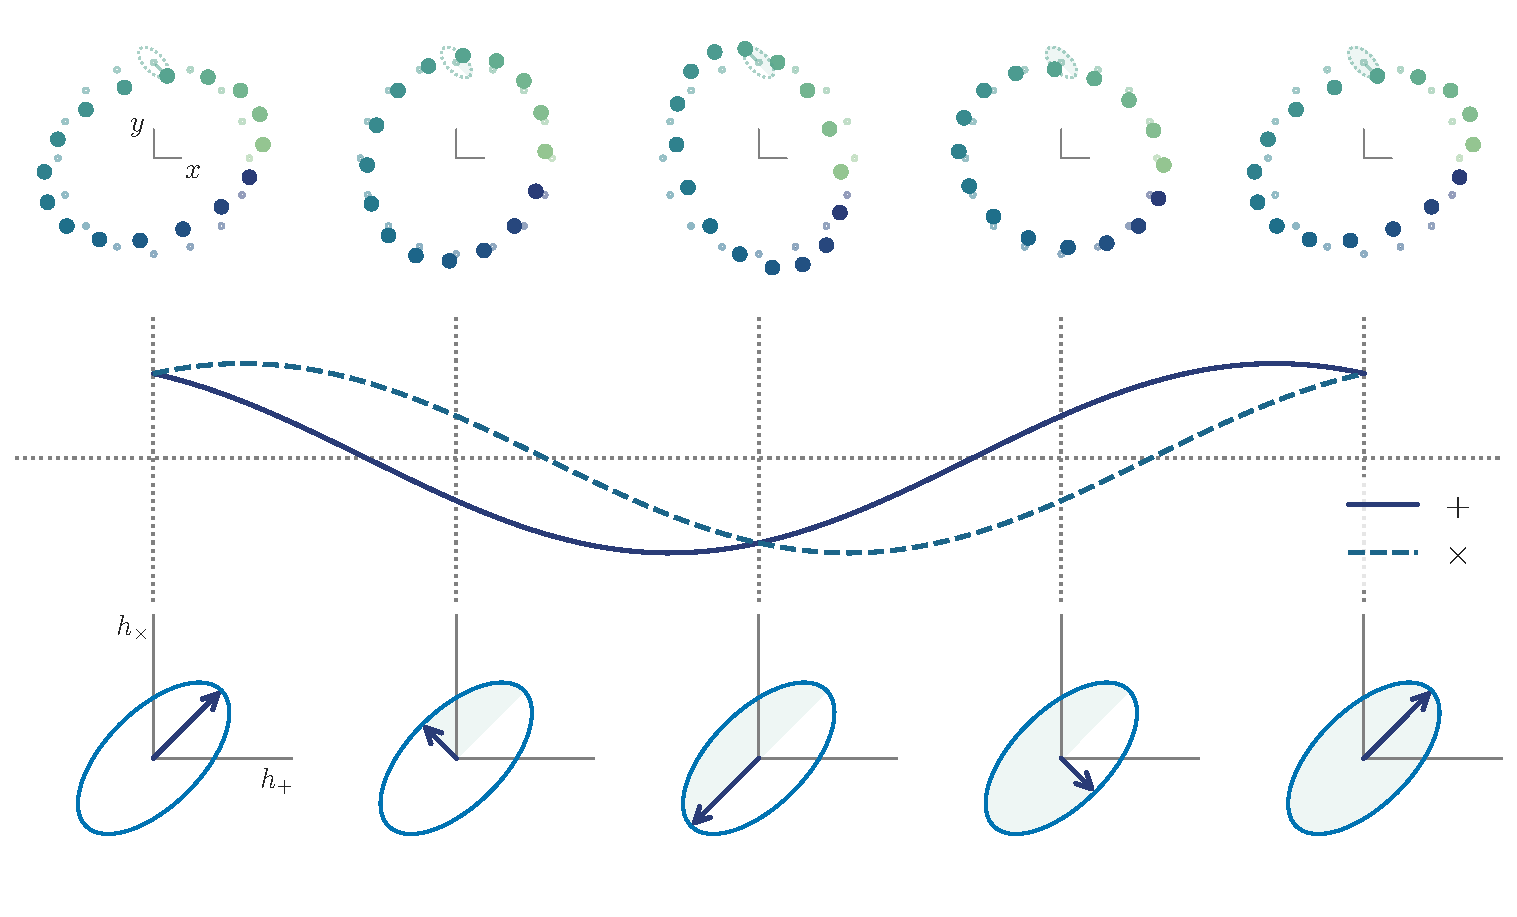
\includegraphics[width=\columnwidth]{pol_diagram_ellip}
\caption{An elliptically polarized GW as a function of time (left to right) over a period, described by Eq.~\eqref{eq:hcomp_ellip} with $\epsilon=1/2$, $\theta=\pi/2$, $\phi=0$ and arbitrary amplitude. \emph{Top:} as the wave propagates out of the page, it deforms a freely falling ring of particles (colored dots) into an ellipsoidal pattern, which in this case rotates counterclockwise with time, albeit nonrigidly; each individual particle is pushed in an ellipse with the same ellipticity as the wave itself, and oriented at an angle $\theta + \varphi$ from the $x$-axis, where $\varphi$ is the polar coordinate locating the particle around the ring.
\emph{Middle:} amplitudes of the plus (solid) and cross (dashed) linear polarizations making up the wave as a function of time.
\emph{Bottom:} representation of the polarization state as a Jones vector in the $+$ and $\times$ space; the phasor rotates counterclockwise as in Fig.~\ref{fig:ellipse}.
}
\label{fig:pol_diagram_ellip}
\end{figure*}

\newcommand{\jonesbasis}{\vec{\mathfrak{e}}}

We can obtain another useful parametrization for fully polarized states by replacing the ellipticity parameter $\epsilon$ in \eq{hcomp_ellip} with an angle $\chi \equiv \arctan \epsilon$, which is also illustrated in Fig.~\ref{fig:ellipse}.
In terms of this quantity and the intensity amplitude $\hat{A}=A\sqrt{1+\epsilon^2}=A \sec\chi$, the elliptical mode of \eq{hcomp_ellip} becomes
\begin{subequations} \label{eq:hcomp_ellip_chi}
\beq
h_+ = \hat{A} \left[\cos\chi \cos \theta \cos(\omega t - \phi) - \sin\chi \sin \theta \sin(\omega t - \phi)\right] ,
\eeq
\beq
h_\times = \hat{A} \left[\cos\chi \sin \theta \cos(\omega t - \phi) + \sin\chi \cos \theta \sin(\omega t - \phi)\right] ,
\eeq
\end{subequations}
Now, $\chi = 0$ gives a linearly polarized state, while $\chi=\pm \pi/4$ gives a R/L circularly polarized state.
Its domain is given by $-\pi/4 \leq \chi \leq \pi/4$, as implied by $-1 \leq \epsilon \leq 1$, and we can further limit $0 \leq \theta \leq \pi$ and $0 \leq \phi \leq \pi$, since Eqs.~\eqref{eq:hcomp_ellip} and\eqref{eq:hcomp_ellip_chi} are invariant under $\{\theta \to \theta + \pi,  \phi \to \phi + \pi\}$.
To accommodate these ranges, it can be useful to work with alternative angles $\bar{\theta} \equiv 2\theta$ and $\bar{\phi} \equiv 2\phi$ that are allowed to range fully over $[0, 2\pi]$.

\subsubsection{Mathematical framework}
\label{sec:math}

The mathematical treatment of polarized GW states is entirely analogous to the electromagnetic case.
To start, any of these states can be represented graphically by series of phasor diagrams like the one in Fig.~\ref{fig:ellipse}, as in the bottom of Figs.~\ref{fig:pol_diagram_circ} and \ref{fig:pol_diagram_ellip}.
For monochromatic modes (i.e., of a definite $\omega$), the same information can also be encoded algebraically in a complex valued \emph{Jones vector} $\vec{C}$ like 
% Any fully-polarized state can be represented by phasor diagrams like the one in Fig.~\ref{fig:ellipse}.
% Additionally, for a monochromatic mode, the time dependence of the phasor can be factored out so that the whole state is encoded in a \emph{Jones vector} $\vec{A}$ like
\beq \label{eq:jones}
\begin{pmatrix}
h_+\\
h_\times
\end{pmatrix} \equiv
\Re \left[ \begin{pmatrix}
C_+\\
C_\times
\end{pmatrix} e^{-i\omega t}\right] \equiv
\Re \left[ \vec{C}\, e^{-i\omega t}\right] ,
\eeq
with $C_{+/\times} \equiv A_{+/\times} \exp(i\phi_{+/\times})$.
In that notation, $ \jonesbasis_+ \equiv \left(1, 0\right)$ encodes a unit-amplitude linearly polarized $+$ mode, and $\jonesbasis_\times \equiv \left(0,1\right)$ a $\times$ mode; meanwhile, $\jonesbasis_{R/L} \equiv \left(1,\pm i\right)/\sqrt{2}$ encode a circular R/L mode, with the plus sign for R.
Thus, the generic signal in \eq{jones} can be equally conveyed by
\beq \label{eq:jones_bases}
\vec{C} = C_+ \, \jonesbasis_+ + C_\times \, \jonesbasis_\times = C_R \, \jonesbasis_R + C_L \, \jonesbasis_L\, ,
\eeq
with $C_{R/L} = (C_+ \mp i C_\times)/\sqrt{2}$ the same complex amplitudes as in \eq{ellip_circ}---although note that here $C_L$ appears without conjugation.
We will briefly make use of Jones vectors to facilitate coordinate transformations below.


Considering the parametrization in \eq{hcomp_ellip_chi}, we have two angles that fully define the shape of the polarization ellipse, $\chi$ and $\theta$.
If we interpret $-\pi/2 \leq 2\chi \leq \pi/2$ and $0 \leq 2\theta \leq 2\pi$ respectively as latitude and longitude coordinates, then the space of all unique polarization states can be arranged into a sphere such that linear polarization states of different orientations live on the equator ($\chi = 0$), and circular states live on the poles ($2\chi = \pm \pi/2$) \cite{poincare,goldstein}.
Any two antipodal states in this so-called \emph{Poincar\'e sphere} can function as a polarization basis.
In this language, reexpressing Eq.~\eqref{eq:planewave} as Eq.~\eqref{eq:planewave_circ} amounted to effecting a Poincar\'{e} rotation of our basis vectors.
The polarization ellipse (Fig.~\ref{fig:ellipse}) can be recovered from the Poincar\'e sphere by a stereographic projection.

If we scale the radius of the Poincar\'{e} sphere to be the signal intensity $I \equiv \hat{A}^2$, then it can be defined in terms of Cartesian coordinates corresponding to the three other \emph{Stokes parameters} that characterize the distribution of power in the signal accross different polarization states \cite{Anile1974}.
For a fully polarized monochromatic mode, in addition to $I$ itself, these are given by
\begin{subequations} \label{eq:stokes}
\beq
Q \equiv |C_+|^2 - |C_\times|^2 = \hat{A}^2 \cos 2\chi \cos 2\theta \, , 
\eeq
\beq
U \equiv C_+ C_\times^* + C_+^* C_\times = \hat{A}^2 \sin2\chi \sin 2\theta \,  ,
\eeq
\beq
V \equiv |C_R|^2 - |C_L|^2 = \hat{A}^2 \sin 2\chi \, ,
\eeq 
\end{subequations}
for $C_+ = (C_R + C_L)/\sqrt{2}$ and $C_\times = i (C_R - C_L)/\sqrt{2}$.
As implied by the definitions above, $Q/I$ controls the (power) fraction of linear polarization, $U/I$ the orientation of the linear component, and $V/I$ the fraction of circular polarization.
The Poincar\'{e} sphere is then the sphere of radius $I$ centered on $\left(Q=0, U=0, V=0\right)$.

For a fully polarized state, the Stokes parameters (quantifying signal power) are equivalent to the polarization quantitites $\left\{A, \epsilon, \theta\right\}$ or $\{\hat{A}, \chi, \theta\}$ defining the ellipse in Fig.~\ref{fig:ellipse} (and quantifying signal amplitude).
Because they are defined in terms of power, Stokes parameters have do not retain phasing information, but have the advantage of being easily generalizable to fully or partially unpolarized waves, which can be achieved by replacing the definition in Eq.~\eqref{eq:stokes} with corresponding two-point correlation functions (power spectra); in the fully-unpolarized case, $Q=U=V=0$ and there is no Poincar\'{e} sphere to speak of.
The Stokes parameters are thus especially useful when dealing with stochastic signals \cite{Romano:2016dpx,Conneely:2018wis,Seto:2008sr,Kato:2015bye}; since we will be dealing mainly with coherent signals, we will not make further reference to Stokes parameters in what follows.

% Consequently, its applicability extends beyond the formal Fourier expansion in \eq{hcomp_fd_rl} to any context in which the signal (or a component thereof) can be described as having a definite polarization state (which may potentially evolve adiabatically).

\subsection{Non-monochromatic modes}
\label{sec:ellip:gen}

% \subsubsection{Fully-polarized non-monochromatic states}

We arrived at the expression for a fully-polarized, monochromatic GW in Eq.~\eqref{eq:hcomp_ellip} by way of the generic Fourier decomposition of a plane wave in Eq.~\eqref{eq:hcomp_fd_rl}, wherein elliptical modes appear naturally with a determinate frequency.
Yet, we may also speak of fully-polarized states even if the signal is not monochromatic.

The argument applies to any high-frequency coherent wave, i.e., any wave that can be written as a slow-varying amplitude modulating a fast phase.
In that case, the polarization parameters $\{A, \epsilon, \theta\}$ can be defined instantaneously using the stationary phase approximation or similar procedures.
This way, any GW with a constant polarization state, i.e., whose polarization ellipse takes a fixed, determinate shape (but not necessarily scale), can be encapsulated by an expression of the form
\begin{subequations} \label{eq:ellip_gen}
\begin{equation} %\label{eq:ellip_sum_p}
h_+ = \mathcal{A}(t) \left[\cos \Phi(t) \cos \theta - \epsilon \sin \Phi(t) \sin\theta \right] ,
\end{equation}
\begin{equation} %\label{eq:ellip_sum_c}
h_\times = \mathcal{A}(t) \left[ \cos \Phi(t) \sin \theta + \epsilon \sin \Phi(t) \cos\theta \right] ,
\end{equation}
\end{subequations}
enhancing Eq.~\eqref{eq:hcomp_ellip} with a (slowly) time varying amplitude $\mathcal{A}(t)$ and a (quickly) time varying phase $\Phi(t)$, which need no longer grow linearly with time.
Following this expression, the aspect ratio and orientation of the polarization ellipse remains constant,%
\footnote{The shape of the ellipse could also be made to vary adiabatically via $\epsilon$ and $\theta$ but that is seldomly done in real-world applications.}
while its size may increase or decrease according to $\mathcal{A}(t)$.
The initial state of the signal is defined by the initial amplitude $A = \mathcal{A}(t=0)$ and phase $\phi = \Phi(t=0)$.

Most conceivable signals are neither monochromatic nor fully polarized.
Nevertheless, a large variety of morphologies can be captured with a finite superposition of elliptically polarized modes, potentially with time-varying polarization parameters as above.
This should be apparent from the fact that an (uncountably) \emph{infinite} set of elliptical modes can describe \emph{any} GW signal, as we showed in \eq{hcomp_fd_rl}.
For many practical applications, it is advantageous to decompose signals into 
sums of fully-polarized modes in the shape of \eq{ellip_gen},
% \begin{subequations}
% \begin{align}
% h_+ = \sum_n A_n(t) &\left[\cos \theta_n \cos(\omega_n t - \phi_n) \right. \\
% &\left. - \epsilon_n \sin \theta_n \sin(\omega_n t - \phi_n)\right] ,\nonumber
% \end{align}
% \begin{align}
% h_\times = \sum_n A_n(t) &\left[\sin \theta_n \cos(\omega t - \phi_n) \right. \\
% &\left.+ \epsilon \cos \theta \sin(\omega t - \phi_n)\right] , \nonumber
% \end{align}
% \end{subequations}
\begin{subequations} \label{eq:ellip_sum}
\begin{equation} \label{eq:ellip_sum_p}
h_+ = \sum \mathcal{A}_n(t) \hspace{-1pt} \left[\cos \Phi_n(t) \cos \theta_n - \epsilon_n \sin \Phi_n(t) \sin\theta_n \right] ,
\end{equation}
\begin{equation} \label{eq:ellip_sum_c}
h_\times = \sum \mathcal{A}_n(t) \hspace{-1pt} \left[ \cos \Phi_n(t) \sin \theta_n + \epsilon_n \sin \Phi_n(t) \cos\theta_n \right] ,
\end{equation}
\end{subequations}
with a sum over some number of modes indexed by $n$, with amplitudes and phases taking some prescribed functional form for each $n$.

The form of Eq.~\eqref{eq:ellip_sum} is flexible enough that it can be used in practice to model arbitrary signals in real detector data.
For example, that is the strategy taken by \textsc{BayesWave} \cite{Cornish:2014kda,Cornish:2020dwh}, which reconstructs generic GW signals by fitting a variable number of elliptically-polarized sine-Gaussians.%
\footnote{\textsc{BayesWave} can currently operate in two configurations: one which assumes the overall signal is elliptically polarized, and another which does not.}
It is also the case, in ringdown studies that fit the final portion of a compact binary signal as a superposition of elliptically polarized damped sinusoids \cite{Isi:2021iql}.

For such applications, each phasing function will usually correspond to some given frequency $\omega_n$ as in a Fourier expansion, so that $\Phi_n(t) = \omega_n t + \phi_n$; meanwhile, the $\mathcal{A}_n(t)$ functions encode amplitude envelopes evolving slowly over some timescale $\tau_n \equiv 1/\gamma_n$ (or, equivalently, with some quality factor $Q_n \equiv \omega_n \tau_n/2$).
For example, in the case of ringdown templates, $\mathcal{A}_n(t) = A_n \exp(-\gamma_n t)$ and $\Phi_n(t) = \omega_n t + \phi_n$, for some set of frequencies and damping rates to be inferred from the data together with polarization parameters $\{ A_n, \epsilon_n, \theta_n, \phi_n\}$.
Equations \eqref{eq:ellip_sum} can be equivalently written in the frequency domain, as done for the sine-Gaussian basis in \cite{Cornish:2014kda,Cornish:2020dwh}.

The elliptical decomposition of Eq.~\eqref{eq:ellip_sum} allows us to flexibly model a GW signal without assuming full independence of the two GW polarizations.
This is justified because, as argued in \cite{Chatziioannou:2021mij}, we expect both polarizations to be generated by the same physical processes, so that their spectral properties should not be totally independent.
Moreover, even if there was a choice of waveframe in which the two linear polarizations looked completely dissimilar, the polarizations will look spectrally similar to generic observers whose frame is randomly oriented (see the discussion of polarization mixing in Sec.~\ref{sec:angles} below).

Besides the modeling of generic signals, \eq{ellip_sum} serves as the exact representation of several classes of astrophysically-relevant signals.
The most salient example of this, as we will see below, is that of CBCs; in particular, a nonprecessing, quasicircular CBC dominated by the quadrupolar angular harmonic of the radiation can be described by a single, fully polarized component, as in \eq{ellip_gen}.

% In fact, as we will see below, the simplest of those signals (viz., nonprecessing inspiral dominated by the quadrupolar angular harmonic) can be described by a single mode like the summand of \eq{hcomp_ellip}, with fixed ellipticity and polarization angle.


\subsection{Relation to spherical harmonics}
\label{sec:harmonics}

When modeling specific sources (e.g., in a numerical-relativity simulation), it is common to decompose the outgoing strain in terms of spin-weighted spherical harmonics ${}_{-2} Y_{\ell m}$ in the frame of the source (e.g., \cite{Kidder:2007rt}), so that, for a detector infinitely far away, we can write
% \begin{align}
% h_+ - i h_\times = \sum_\ell \sum_{m>0} &\left[ H_{\ell m}(t)\, {}_{-2}Y_{\ell m} (\iota, \varphi) + \right. \nonumber \\
% &\left. H_{\ell-m}(t)\, {}_{-2}Y_{\ell -m} (\iota, \varphi) \right]
% \end{align}
\begin{align} \label{eq:spherical}
H(t) = \sum_{\ell \geq 2} \sum_{-\ell \leq m \leq \ell} H_{\ell m}(t)\, {}_{-2}Y_{\ell m} (\iota, \varphi)\, ,
\end{align}
for a source seen with inclination $\iota$ and azimuthal angle $\varphi$, with intrinsic time-dependence encoded in the $H_{\ell m}$ functions as determined by Einstein's equations.
The decomposition into spherical harmonics presumes the choice of both (1) a polar frame defining $\iota$ and $\varphi$, and (2) an orientation of the waveframe vectors with respect to the direction of propagation to establish the meaning of $h_{+/\times}$ as in \eq{hij}.
In the LIGO convention (which follows \cite{Blanchet:2008je,Faye:2012we}), the waveframe in \eq{spherical} is defined by $\hat{x} = -\hat{e}_\iota$ and $\hat{y} = - \hat{e}_\varphi$ \cite{LALSuite:source}, and the overall polar frame is centered on and comoving with the source, with an orientation following its symmetries (e.g., aligned with the orbital plane).

The different $H_{\ell m}$'s in \eq{spherical} are generated by the time evolution of specific current and mass moments of the source \cite{Thorne:1980ru}.
As such, their structure must inherit the symmetries of Einstein's equations, including parity.
In particular, for any source satisfying equatorial-reflection (planar) symmetry, like a nonprecessing inspiral, parity can be shown to imply that $H_{\ell -m} = (-1)^\ell H_{\ell m}^*$ \cite{Faye:2012we}, assuming that the coordinates in \eq{spherical} are oriented such that $\iota=\pi$ is the plane of symmetry.
Allowing for a generic (slow) amplitude and (fast) phase evolution by writing $H_{\ell m}(t) = \mathcal{A}_{\ell m}(t) \exp[-i \Phi_{\ell m}(t)]$, this symmetry reduces to $\mathcal{A}_{\ell -m}(t) = (-1)^\ell \mathcal{A}_{\ell m}(t)$ and $\Phi_{\ell m}(t) = - \Phi_{\ell -m}(t)$, where we have taken $\mathcal{A}$ and $\Phi$ to be real valued.
In that case, \eq{spherical} can be rewritten with an explicit term for negative values of $m$ as
\begin{widetext}
\begin{subequations} \label{eq:spherical_modes}
\begin{align}
H(t) &= \sum_{\ell \geq 2} \sum_{0\leq m \leq \ell} \left[H_{\ell m}(t)\, {}_{-2}Y_{\ell m} (\iota, \varphi) + H_{\ell -m}(t)\, {}_{-2}Y_{\ell -m} (\iota, \varphi) \right] \\
%&= \sum_{\ell \geq 2} \sum_{0\leq m \leq \ell} \left[\mathcal{A}_{\ell m}(t)\, e^{-i\Phi_{\ell m} (t)} {}_{-2}Y_{\ell m}(\iota, \varphi) +  (-1)^\ell \mathcal{A}_{\ell m}(t)\, e^{i\Phi_{\ell m} (t)} {}_{-2}Y_{\ell- m}(\iota, \varphi) \right] \\
&= \sum_{\ell \geq 2} \sum_{0\leq m \leq \ell} \left[\mathcal{A}_{\ell m}(t)\, e^{-i\Phi_{\ell m} (t)} {}_{-2}Y_{\ell m}(\iota, \varphi) +  \mathcal{A}_{\ell m}(t)\, e^{i\Phi_{\ell m} (t)} {}_{-2}Y_{\ell m}^*(\pi-\iota, \varphi) \right] \\
&= \sum_{\ell \geq 2} \sum_{0\leq m \leq \ell} \left[\mathcal{C}_{\ell m}(t)\, e^{-i\Phi_{\ell m} (t)}  +  \mathcal{C}_{\ell -m}(t)\, e^{i\Phi_{\ell m} (t)} \right]\, ,
\end{align}
\end{subequations}
\end{widetext}
for some overall complex-valued amplitudes $\mathcal{C}_{\ell \pm m}$, absorbing the angular dependence of the spherical harmonics and any potential (slow) time variation in $\mathcal{A}_{\ell m}$.
In the second line above, we took advantage of the identity relating spherical harmonics for different signs of $m$, ${}_{-2} Y_{\ell -m}(\iota,\varphi) = (-1)^{\ell} {}_{-2} Y_{\ell m}^*(\pi-\iota,\varphi)$ \cite{goldberg:1967}.

% % The different $H_{\ell m}$'s in \eq{spherical} are generated by the time evolution of specific current and mass moments of the source, and, therefore, are often associated with specific signal frequencies \cite{Thorne:1980ru}.
% For example, the dominant $\ell= |m|=2$ mode in a nonprecessing compact binary inspiral will evolve with a signal freqyency $\omega_{22}$ which is twice the orbital frequency $\omega_\mathrm{orb}$ or, more generally for other harmonics, $\omega_{\ell m} = m\, \omega_\mathrm{orb}$, with parity invariance requiring $\omega_{\ell m}= - \omega_{\ell - m}$.
% If that harmonic structure holds, then Eq.~\eqref{eq:spherical} is equivalent to the elliptical decomposition of Eq.~\eqref{eq:ellip_sum}, as we proceed to show.
% 
% For concreteness, represent the $H_{\ell m}$ schematically as simple monochromatic components $H_{\ell m} (t) = \mathcal{C}_{\ell m} \exp\left(-i \omega_{\ell m} t\right)$, where $\mathcal{C}_{\ell m}$ is some complex-valued amplitude, that could be varying slowly with time (slower than $\omega_{\ell m}$).
% We can then refactor Eq.~\eqref{eq:spherical} so that we only sum over nonnegative values of $m$,
% \begin{widetext}
% \begin{subequations} \label{eq:spherical_modes}
% \begin{align}
% h_+ - i h_\times &= \sum_{\ell \geq 2} \sum_{0\leq m \leq \ell} \left[H_{\ell m}(t)\, {}_{-2}Y_{\ell m} (\iota, \varphi) + H_{\ell -m}(t)\, {}_{-2}Y_{\ell -m} (\iota, \varphi) \right] \\
% &= \sum_{\ell \geq 2} \sum_{0\leq m \leq \ell} \left[\mathcal{C}_{\ell m} e^{-i\omega_{\ell m} t} {}_{-2}Y_{\ell m}(\iota, \varphi) +  \mathcal{C}_{\ell -m} e^{i\omega_{\ell m} t} {}_{-2}Y_{\ell- m}(\iota, \varphi) \right] \\
% &= \sum_{\ell \geq 2} \sum_{0\leq m \leq \ell} \left[C_{\ell m} e^{-i\omega_{\ell m} t}  +  C_{\ell -m} e^{i\omega_{\ell m} t} \right]\, ,
% \end{align}
% \end{subequations}
% \end{widetext}
% where, in the last line, we have absorbed the angular factors into $C_{\ell m} \equiv {}_{-2}Y_{\ell m} (\iota, \varphi)\, \mathcal{C}_{\ell m}$.

The summand in the last line of \eq{spherical_modes} takes the form of \eq{ellip_circ}, and its interpretation is the same for any fixed observation direction: each $(\ell$, $|m|)$ angular harmonic contributes a single, elliptically polarized mode to the waveform.
Thus the overall strain for such a source must be a superposition of purely polarized modes, with adiabatically evolving amplitudes as in \eq{ellip_sum}.

The amplitude and ellipticity of each mode are determined by a combination of the intrinsic amplitudes $\mathcal{H}_{\ell \pm m}$, and the viewing angle $(\iota, \varphi)$---the latter through the ${}_{-2} Y_{\ell m}$ factors.
The intensity of the mode will vary with time following $\mathcal{A}_{\ell m}(t)$; meanwhile, its ellipticity, as observed from a given $\iota$ and $\varphi$, will be fixed by the relative amplitudes of the $\pm|m|$ spherical harmonics,
\begin{align}
%\epsilon_{\ell|m|}(\iota, \varphi) = \frac{\left|{}_{-2} Y_{\ell m}(\iota,\varphi)\right| - \left|{}_{-2} Y_{\ell m}^*(\pi-\iota,\varphi)\right|}{\left|{}_{-2} Y_{\ell m}(\iota,\varphi)\right| + \left|{}_{-2} Y_{\ell m}^*(\pi-\iota,\varphi)\right|} \\
\epsilon_{\ell|m|}(\iota) = \frac{\left|{}_{-2} Y_{\ell m}(\iota,\varphi)\right| - \left|{}_{-2} Y_{\ell -m}(\iota,\varphi)\right|}{\left|{}_{-2} Y_{\ell m}(\iota,\varphi)\right| + \left|{}_{-2} Y_{\ell -m}(\iota,\varphi)\right|} ,
\end{align}
which is exclusively a function of the inclination $\iota$, because $\varphi$ only affects the phase (not the magnitude) of the spin-weighted spherical-harmonic factors, with ${}_{-2} Y_{\ell m}(\iota,\varphi) = {}_{-2} Y_{\ell m}(\iota) \exp(i m \varphi)$ factoring out the $\varphi$ dependence.

% Although we have simplified \eq{spherical_modes} by taking each $(\ell, m)$ mode to be monochromatic, we would have arrived at the same conclusion regarding polarizations had we instead allowed for a generic (slow) amplitude and (fast) phase evolution by writing $H_{\ell m}(t) = \mathcal{A}_{\ell m}(t) \exp[-i \Phi_{\ell m}(t)]$, for real valued $\mathcal{A}_{\ell m}$ and with parity invariance now requiring $\Phi_{\ell m}(t) = - \Phi_{\ell -m}^*(t)$; in that case the last line of \eq{spherical_modes} would have taken the form of \eq{ellip_sum}, with each summand representing a fully polarized, albeit non-monochromatic, mode.

The complex strain $H_{\ell|m|}(t)$ for a given elliptical $(\ell, |m|)$ mode, as given by the summand in \eq{spherical_modes}, can be further rewritten as
\begin{equation}
H_{\ell|m|}(t) = \mathcal{A}_{\ell m}(t) \left[ Y^+_{\ell m} \cos \Phi_{\ell m}'(t) - 
i Y^\times_{\ell m} \sin \Phi_{\ell m}'(t) \right],
\end{equation}
where we have defined $\Phi_{\ell m}'(t) \equiv \Phi_{\ell m}(t) - m \varphi$, and
\begin{equation}
Y_{\ell m}^{+/\times}(\iota) \equiv {}_{-2} Y_{\ell m}(\iota) \pm {}_{-2} Y_{\ell m}(\pi-\iota) \, ,
\end{equation}
with the plus (minus) sign for $+$ ($\times$), and noting that, after factoring out the $\varphi$ dependence, the ${}_{-2} Y_{\ell m}(\iota)$ factors are real valued.
For the special case of the dominant $\ell=|m|=2$ mode, the strain $H_{\ell|m|} = h_+ - i h_\times$ thus reduces to
\begin{subequations} \label{eq:nonprecessing}
\beq
h_+ = \frac{1}{2} \sqrt{\frac{5}{4\pi}} \mathcal{A}_{22}(t) \left(1 + \cos^2\iota\right) \cos \Phi'_{22}(t) \, , 
\eeq
\beq
h_\times = \sqrt{\frac{5}{4\pi}} \mathcal{A}_{22}(t)  \cos\iota \sin \Phi'_{22}(t) \, ,
\eeq
\end{subequations}
as can be checked by computing explicit expressions for ${}_{-2} Y_{22}(\iota)$.
This is exactly of the form of \eq{ellip_gen}, with amplitude $\mathcal{A} = \sqrt{5/16\pi}\,\mathcal{A}_{22}\left(1+\cos^2\iota\right)$, ellipticity
\beq \label{eq:ellip_cosi}
\epsilon = \frac{2 \cos\iota}{1+\cos^2\iota}\, ,
\eeq
which we illustrate in Fig.~\ref{fig:ellip_cosi}, and $\theta = 0$.
The fact that $\theta = 0$ is a consequence of our special choice of coordinate frame in \eq{spherical}, which we constructed to reflect the symmetries of the planar source so that the equator is the plane of symmetry (we return to this point in Sec.~\ref{sec:position}).

\begin{figure}
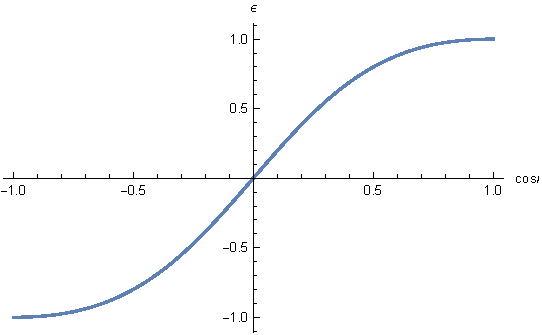
\includegraphics[width=\columnwidth]{ellip_cosi}
\caption{Ellipticity ($\epsilon$, ordinate) as a function of the cosine of the inclination ($\cos\iota$, abscissa) for the $\ell = |m| = 2$ GW strain from a nonprecessing compact binary inspiral, Eq.~\eqref{eq:ellip_cosi}. The signal from a face-on (face-off) binary has ellipticity $\epsilon = +1$ ($\epsilon=-1$), meaning it has a right-handed (left-handed) circular polarization; an edge-on source has a linear polarization.}
\label{fig:ellip_cosi}
\end{figure}

The above results, Eqs.~(\ref{eq:spherical_modes}--\ref{eq:ellip_cosi}), hold only for source with equatorial-reflection symmetry.
The GWs for more generic, precessing, sources will not generally be given by the superposition of fully polarized modes with constant ellipticity.
However, some of such signals may be decomposed into elliptical modes of slowly evolving ellipticity; that is the case, for example, for the early stages of precessing compact binary inspirals, whose signal can be well approximated by \eq{nonprecessing} with a slowly time varying inclination.

In some cases, nonplanar sources can also give rise to superpositions of fully polarized modes.
For example, this is the case for black-hole ringdown signals \cite{Vishveshwara:1970cc, Press:1971wr, Teukolsky:1973ha, Chandrasekhar:1975zza}, which can be written as a harmonic expansion similar to \eq{spherical},
\beq \label{eq:spheroidal}
H(t) = \sum_{\ell \geq 2} \sum_{-\ell \leq m \leq \ell} \sum_{n\geq 0} C_{\ell m n} e^{-i\tilde{\omega}_{\ell m n} t} {}_{-2}S_{\ell m n} (\iota, \varphi) ,
\eeq
for complex frequencies $\tilde{\omega}_{\ell m n} \equiv \omega_{\ell m n} - i/\tau_{\ell m n}$ indexed by the usual angular numbers $\ell$ and $m$, as well as an overtone number $n$, which orders modes of a given $(\ell, m)$ by decreasing damping time; the angular dependence is encoded in the spin-weighted spheroidal harmonics, ${}_{-2}S_{\ell m n}$ \cite{Teukolsky:1973ha,Press:1973zz,Leaver:1985ax,Berti:2005gp,Cook:2014cta}, which have replaced the spherical harmonics in \eq{spherical}.
Parity in this decomposition implies $\tilde{\omega}_{\ell m n} = -\tilde{\omega}_{\ell-m n}^*$; it can thus be shown that, for fixed $\iota$ and $\varphi$, \eq{spheroidal}, is equivalent to
\beq \label{eq:ringdown}
H(t) = \sum \left( C_{\ell m n}' e^{-i\omega_{\ell m n} t} + C_{\ell -m n}' e^{i\omega_{\ell m n} t} \right) e^{-t/\tau_{\ell m n}} ,
\eeq
where the $m$ sum is now restricted to nonnegative values, $0 \leq m \leq \ell$, and $C'_{\ell \pm m n}$ are redefined amplitudes absorbing angular factors.
Comparing to \eq{ellip_circ}, it is evident from \eq{ringdown} that the ringdown strain is made up from elliptically polarized components, with exponentially decaying amplitudes.
If the ringdown excitations had equatorial symmetry, then the initial amplitudes in \eq{spheroidal} would satisfy $C_{\ell -m n }= (-1)^{\ell} C^*_{\ell m}$, and the ellipticity of the observed modes would only be a function of the observing direction.
(See Sec.~IIA and Appendix B of \cite{Isi:2021iql} for an extended discussion.)


\section{Polarization angles}
\label{sec:angles}

\subsection{Wave-frame and the angle $\psi$}
\label{sec:pol}

Equation \eqref{eq:hij} presumes a specific choice of frame orientation that defines the basis in which the $h_{ij}$ components are written and, therefore, the physical meaning of $h_{+}$ and $h_\times$.
Although \eq{hij} requires that $\hat{z}$ be parallel to the (spatial) wave vector $\vec{k}$, there is no a priori restriction on the orientation of the $x$ and $y$ axes within the plane perpendicular to $\vec{k}$.
This freedom is usually encapsulated in the choice of an arbitrary \emph{polarization angle} $\psi$, defined with respect to some convenient reference direction.
For instance, in the LIGO convention, this angle is defined with respect to celestial coordinates such that $\psi=0$ means that the waveframe $\hat{x}$ is parallel to the celestial equator due west, and $\psi$ is measured following the right hand rule around $\hat{z}$ \cite{LALSuite:wave}; we illustrate this in Fig.~\ref{fig:diagram_waveframe}.

With some trigonometry, it is straightforward to show that a \emph{clockwise}%
\footnote{This clockwise \emph{passive} rotation of the waveframe corresponds to a counterclockwise \emph{active} rotation of the polarization state.}
rotation of $\hat{x}$ and $\hat{y}$ by some angle $\Delta \psi$ around $\hat{z}$ leaves the form of \eq{hij} unchanged after redefining
\begin{subequations} \label{eq:htransf}
\beq
h_+ \rightarrow h_+' = h_+ \cos 2\Delta \psi - h_\times \sin 2\Delta\psi \, ,
\eeq
\beq
h_\times \rightarrow h_\times' = h_\times \cos 2\Delta \psi + h_+ \sin 2\Delta\psi \, .
\eeq
\end{subequations}
This contravariant transformation gives the polarization amplitudes that would be measured by an observer in the rotated (primed) frame, as a function of the amplitudes in the original frame.
The $2\Delta\psi$ dependence in \eq{htransf} reveals the fact that $h_+$ and $h_\times$ are nothing but the two components of a tensor field with spin-weight $|s|=2$, and the two polarizations are only defined up to an arbitrary choice of $\psi$.

The basis polarization tensors themselves transform inversely to the amplitudes, covariant with the rotation.
Under clockwise rotations of the wave frame, therefore, the antenna patterns of \eq{h} transform through an expression complementary to \eq{htransf},
\begin{subequations} \label{eq:Ftransf}
\beq
F_+ \rightarrow F_+' = F_+ \cos 2\Delta \psi + F_\times \sin 2\Delta\psi \, ,
\eeq
\beq
F_\times \rightarrow F_\times' = F_\times \cos 2\Delta \psi - F_+ \sin 2\Delta\psi \, ,
\eeq
\end{subequations}
ensuring that the observable $h(t)$ in \eq{h} is independent of the arbitrary angle $\psi$.
More generally, any scalar like $D^{ij} e^{p}_{ij}$ will necessarily be frame invariant.%
\footnote{This extends to gauge transformations: the spacetime tensors $D_{ab}$ and $h_{ab}$ are gauge dependent, but their innerproduct is not.}

Unlike the linear modes of Eq.~\eqref{eq:lin}, the tensors of Eq.~\eqref{eq:circ} do not mix under rotations around the direction of propagation:
the circular polarizations are eigenstates of the helicity operator with weight $\pm 2$, corresponding to the two helicities of a spin-2 massless particle (see, e.g., \cite{Hinterbichler2011}).
The equivalent transformation to Eq.~\eqref{eq:htransf} is
\begin{subequations} \label{eq:htransf_circ}
\begin{align}
h_R &\rightarrow h_R' = h_R \exp(- i2  \Delta \psi) \, ,\\
h_L &\rightarrow h_L' = h_L \exp(+ i2  \Delta \psi)\, ,
\end{align}
\end{subequations}
meaning that a rotation around $\hat{z}$ is equivalent to a simple change in the overall phase of the circular polarization components.
As such, a change in $\psi$ can be absorbed by a redefinition of the Fourier phases in \eq{hcomp_fd_rl}, multiplying the integral through by $\exp(-i2\Delta\psi)$.

\begin{figure}
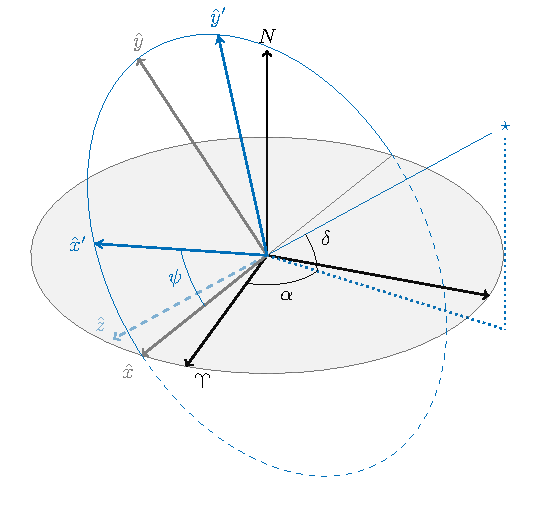
\includegraphics[width=0.9\columnwidth]{diagram_waveframe.pdf}
\caption{Standard construction of the polarization waveframe used in LIGO-Virgo data analysis \cite{LALSuite:wave}. Earth sits at the origin of the equatorial coordinate system defined by the celestial north ($N$) and the vernal equinox ($\vernal$). The sky location of a source ($\star$) is encoded in its right ascension ($\alpha$) and declination ($\delta$), so that the wave propagation direction is $\hat{k}=\hat{z}=-(\cos\delta \cos\alpha, \cos\delta\sin\alpha, \sin\delta)$. The canonical polarization frame is defined by $\hat{x}'=(\sin\alpha, -\cos\alpha,0)$ as being the intersection between the plane of the sky (blue circle) and the celestial equator (gray circle), and $\hat{y}'=(-\sin\delta \cos\alpha, \sin\delta\sin\alpha, \cos\delta)$ the projection of $N$ onto the plane of the sky, completing the right-handed basis with $\hat{z}$.
In terms of these vectors, an arbitrary polarization frame rotated by some angle $\psi$ around $\hat{z}$ is given by $\hat{x}=\cos\psi\,\hat{x} + \sin\psi\,\hat{y}$ and $\hat{y}=-\sin\psi\,\hat{x} + \cos\psi\,\hat{y}$. (Dashed trace indicates elements below the equator.)}
\label{fig:diagram_waveframe}
\end{figure}

Equations~(\ref{eq:htransf}--\ref{eq:htransf_circ}) allow us to transform predictions for the strain $h_{ij} = h_+ e^{+}_{ij} + h_{\times} e^{\times}_{ij}$ in some waveframe $\{\hat{x}, \hat{y}, \hat{z}\}$ to a different one $\{\hat{x}', \hat{y}', \hat{z}'\}$, rotated clockwise around $\hat{k}=\hat{z}=\hat{z}'$ by $\Delta \psi$ (simply labeled $\psi$, if the primed frame corresponds to the reference frame defining $\psi=0$).
In real-world data analysis applications, however, we simply write the unprimed basis vectors in the primed basis and evaluate \eq{h} through numerical dot products using \eq{lin}.
To do this, we express the components of $e^{+/\times}_{ij}$ and $D_{ij}$ in a common basis suitably aligned with the reference waveframe---for ground-based detectors, where we take $\hat{x}'$ to be parallel to the celestial equator, these are equatorial celestial coordinates (Fig.~\ref{fig:diagram_waveframe}).
Knowing how the $\{\hat{x}', \hat{y}'\}$ vectors are expressed in such coordinates, we can construct $h_{ij}'$ by noting that $\hat{x} = \cos\psi\, \hat{x}' + \sin\psi\, \hat{y}'$ and $\hat{y}= - \sin\psi\, \hat{x}' + \cos\psi\, \hat{y}'$.
It is then straightforward to write the signal at any given detector in terms of the polarization amplitudes $h_{+/\times}$ computed in the original frame.

The definition of the angle $\psi$ (as in Fig.~\ref{fig:diagram_waveframe}) is not intrinsically related to any feature of the signal: it simply chooses an absolute reference direction that defines an arbitrary frame in which to prescribe the $h_+$ and $h_\times$ polarization functions in \eq{hij}, or equivalently, the frame in which to measure the phases of the circularly polarized Fourier components.
Nevertheless, even though any choice of assignment for $\psi$ is formally valid, specific signal morphologies may make some choices more convenient than others.

\subsection{Elliptical waves and the angle $\theta$}
\label{sec:ellip}

\begin{figure}[tbp]
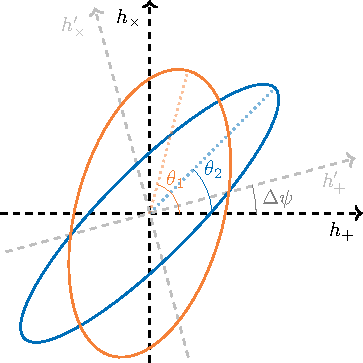
\includegraphics[width=0.65\columnwidth]{diagram_ellipse_extra.pdf}
\caption{A clockwise rotation of the physical waveframe of Fig.~\ref{fig:diagram_waveframe} by an angle $\Delta\psi$ manifests as a rotation by $2\Delta\psi$ in the $(h_+,h_\times)$ polarization space, so that elliptical modes with original orientation angles $\theta_n$ are seen to have orientations $\theta_n'=\theta_n + 2\Delta\psi$ in the new (primed) frame.
The diagram illustrates two such modes with ellipse orientations $\theta_{1/2}$ with respect to $h_+$, and  $\theta_{1/2}'$ with respect to $h_+'$.
}
\label{fig:diagram_ellipse_extra}
\end{figure}

Another notion of ``polarization angle'' arises naturally in the description of elliptically polarized signals.
The expression for an elliptical wave in \eq{ellip_gen} presumes some specific choice of $\psi$ that defines the meaning of plus vs cross by orienting $\hat{x}$, as explained in the previous section.
The expression simplifies if we choose that angle such that the plus and cross axes are aligned with the principal components of the ellipse, i.e., constructing the polarization frame to ensure that $\theta = 0$ (see Fig.~\ref{fig:ellipse}).

With such a choice of wave frame (equivalently, choice of $\psi$), \eq{ellip_gen} becomes just
\begin{subequations} \label{eq:ellip_frame}
\beq
h_+ = \mathcal{A}(t) \cos \Phi(t) \, ,
\eeq
\beq
h_\times = \epsilon \mathcal{A}(t) \sin \Phi(t)\, ,
\eeq
\end{subequations}
and we may just read off the ellipticity as the ratio of the $\times$ to $+$ amplitudes.
Crucially, an elliptical wave will generally not take the form of Eq.~\eqref{eq:ellip_frame} unless $\hat{x}$ is chosen appropriately; only circularly polarized signals ($\epsilon=\pm1$) will take  this simplified form irrespective of the wave frame orientation (again showing that these are eigenstates of the helicity operator).

Therefore, when working with a single elliptically-polarized wave, Eq.~\eqref{eq:ellip_frame} defines a privileged orientation of the wave frame, unique up to rotations by $\pi/2$ around $\hat{z}$.
If we adopt $\theta =0$ as a convention (or, equivalently, $\theta=\pi$), then we \emph{define} our wave frame to lie along the principal axes of the polarization ellipse and, thus, the polarization angle $\psi$ becomes synonymous with the polarization ellipse orientation.
However, the two angles $\theta$ and $\psi$ are conceptually distinct; in particular, $\theta$ is defined only for elliptically polarized waves, whereas $\psi$ is always defined.

As for any GW, the detector output for an elliptically polarized wave will be given by \eq{h}.
In this case, however, \eq{Ftransf} implies that $\psi$ and $\theta$ are degenerate, as detailed in Appendix A of \cite{Isi:2017equ}.
Concretely, for a fixed sky location (i.e., propagation direction), rotating the waveframe \emph{clockwise} around $\hat{z}$ results in a change from $\psi \to \psi' = \psi + \Delta\psi$ in the antenna patterns, which can be absorbed by a change in $\theta$.
This is because the expression for the strain at a given detector,
\beq
h = F_+(\psi + \Delta \psi)\, h_+ + F_\times(\psi + \Delta \psi)\, h_\times \, ,
\eeq
can be expanded by means of \eq{Ftransf} to read
\begin{align}
h = &\left[ F_+(\psi) \cos 2\Delta\psi + F_\times(\psi) \sin 2\Delta\psi \right] h_+\, + \\
 &\left[F_\times(\psi) \cos 2\Delta\psi - F_+(\psi)\sin 2\Delta\psi\right] h_\times \, .
\end{align}
Plugging in the expressions for an elliptical wave in \eq{ellip_gen} and taking advantage of trigonometric identities, this can be rearranged into
\begin{widetext}
\begin{align} \label{eq:theta_psi}
h = & \mathcal{A}(t) \left[\cos \Phi(t) \cos(\theta + 2\Delta\psi) -  \epsilon \sin \Phi(t)\sin(\theta + 2\Delta\psi) \right] F_+(\psi) +\nonumber\\
&\mathcal{A}(t) \left[\cos \Phi(t) \sin(\theta + 2\Delta\psi) + \epsilon \sin \Phi(t) \cos(\theta + 2\Delta\psi) \right] F_\times(\psi), 
\end{align}
\end{widetext}
which is the same result we would have obtained by replacing $\theta \to \theta' = \theta + 2 \Delta\psi$ in \eq{ellip_gen};
for a signal made up of multiple fully-polarized components, as in \eq{ellip_sum}, the waveframe orientation affect all ellipse orientations in the same way, i.e., $\theta_n \to \theta_n'=\theta_n + \Delta\psi$ (Fig.~\ref{fig:diagram_ellipse_extra}).
We could have equivalently (and more quickly) derived this by noting that $\theta$ is related to the phases of the circularly-polarized components of the signal by $\theta = \left(\phi_L - \phi_R\right)/2$, as in \eq{hcomp_ellip}; the transformation rule for $\theta$ then follows from \eq{htransf_circ}, which implies $\phi_{R/L} \to \phi'_{R/L} \mp 2\Delta\psi$, with the negative (positive) sign for R (L).

This implies that elliptical-wave analyses that allow $\theta$ to vary freely should avoid degeneracies by fixing $\psi$ to an arbitrary a priori value.
Choosing this fiducial value to be $\psi=0$, the template at a given detector would be constructed as
\begin{equation}
h = F_+(\psi=0)\, h_+ + F_\times(\psi=0)\,  h_\times \, ,
\end{equation}
for $h_{+/\times}$, as in Eq.~\eqref{eq:ellip_sum}, functions of $\{\theta_i, \epsilon_i\}$ and whatever other parameters are needed to evaluate the amplitude and phasing functions $\{\mathcal{A}_i(t), \Phi_i(t)\}$ (or their frequency-domain analogs).
The antenna patterns $F_{+/\times}$ are evaluated for some sky location and arrival time, which can be allowed to vary to be measured from the data.
On the other hand, the angle $\psi$ is fixed; allowing it to vary would amount to shifting all $\theta_i$ values by $2\psi$, per Eq.~\eqref{eq:theta_psi}.
Fixing $\psi$ to some fiducial value was the approach taken in \cite{Isi:2017equ,Chatziioannou:2021mij,Isi:2021iql}.



% \begin{alignat}{2}
% h &= &&\left. F_+(\psi + \Delta \psi) h_+ + F_\times(\psi + \Delta \psi) h_\times\right.  \\
%   &= &&\left[ F_+(\psi) \cos 2\Delta\psi + F_\times(\psi) \sin 2\Delta\psi \right] h_+\, + \\
% & &&\left[F_\times(\psi) \cos 2\Delta\psi - F_+(\psi)\sin 2\Delta\psi\right] h_\times, 
% \end{alignat}
% The (arbitrary) choice to set $\psi=0$ in the antenna pattern evaluation is legitimate because that degree of freedom is fully degenerate with the $\theta_i$ via Eq.~\eqref{eq:Ftransf}, as detailed in Appendix A of \cite{Isi:2017equ}.
% Concretely, a change from $\psi = 0$ to $\psi= \Delta\psi$ can be written as
% \begin{align}
% h = &\left[ F_+(\psi=0) \cos 2\Delta\psi + F_\times(\psi=0) \sin 2\Delta\psi \right] h_+\, +\nonumber\\
% &\left[F_\times(\psi=0) \cos 2\Delta\psi - F_+(\psi=0)\sin 2\Delta\psi\right] h_\times, 
% \end{align}
% suppressing the sky location dependence for simplicity.

% \begin{align}
% h = & \left[h_+ \cos 2\Delta\psi - h_\times \sin 2\Delta\psi \right] F_+(\psi=0) +\nonumber\\
% &\left[h_\times \cos 2\Delta\psi + h_+ \sin 2\Delta\psi\right] F_\times(\psi=0), 
% \end{align}

% \begin{widetext}
% \begin{align}
% h = & \left[A(t) \left[\cos \Phi(t) \cos \theta - \epsilon \sin \Phi(t) \sin\theta \right] \cos 2\Delta\psi - A(t) \left[ \cos \Phi(t) \sin \theta + \epsilon \sin \Phi(t) \cos\theta \right]  \sin 2\Delta\psi \right] F_+(\psi=0) +\nonumber\\
% &\left[A(t) \left[ \cos \Phi(t) \sin \theta + \epsilon \sin \Phi(t) \cos\theta \right]  \cos 2\Delta\psi + A(t) \left[\cos \Phi(t) \cos \theta - \epsilon \sin \Phi(t) \sin\theta \right] \sin 2\Delta\psi\right] F_\times(\psi=0), 
% \end{align}
% \end{widetext}

% \begin{widetext}
% \begin{align}
% h = & A(t) \left[\cos \Phi(t) \left[ \cos 2\Delta\psi\cos \theta - \sin \theta \sin 2\Delta\psi  \right] -  \epsilon  \sin \Phi(t)\left[ \cos 2\Delta\psi \sin\theta+ \cos\theta \sin 2\Delta\psi\right] \right] F_+(\psi=0) +\nonumber\\
% &A(t) \left[\cos \Phi(t) \left[\sin \theta \cos 2\Delta\psi + \cos \theta \sin 2\Delta\psi \right] + \epsilon \sin \Phi(t) \left[\cos\theta \cos 2\Delta\psi - \sin\theta \sin 2\Delta\psi \right] \right] F_\times(\psi=0), 
% \end{align}
% % \end{widetext}
% 
% % \begin{widetext}
% \begin{align}
% h = & A(t) \left[\cos \Phi(t) \cos(\theta + 2\Delta\psi) -  \epsilon \sin \Phi(t)\sin(\theta + 2\Delta\psi) \right] F_+(\psi=0) +\nonumber\\
% &A(t) \left[\cos \Phi(t) \sin(\theta + 2\Delta\psi) + \epsilon \sin \Phi(t) \cos(\theta + 2\Delta\psi) \right] F_\times(\psi=0), 
% \end{align}
% \end{widetext}
% 

\subsection{Compact binaries and the angles $\Psi$ and $\Omega$}
\label{sec:position}

\begin{figure}
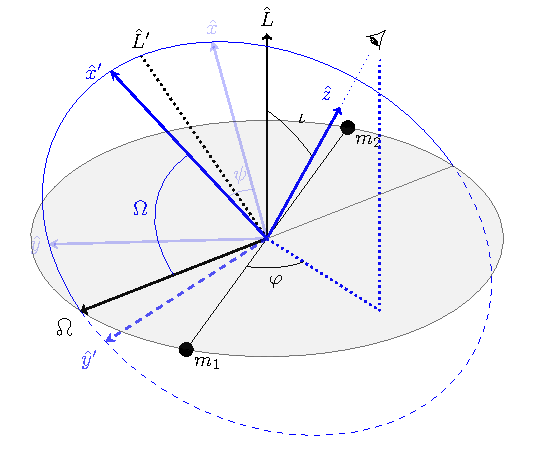
\includegraphics[width=0.9\columnwidth]{diagram_sourceframe.pdf}
\caption{Standard construction of the source frame used in LIGO-Virgo data analysis of compact binaries \cite{LALSuite:source}. Two inspiraling objects ($m_1$ and $m_2$) define an orbital plane (gray disk) perpendicular to the orbital angular momentum direction $\hat{L}$. At a given time (say, when the observed GW signal reaches 20 Hz) observers on Earth will be oriented with an inclination $\iota$ relative to $\hat{L}$ and an azimuthal angle $\varphi$ with respect to the line from $m_2$ to $m_1$ (related to the reference orbital phase $\Phi=\pi/2-\varphi$).
The intersection between the orbital plane and the plane of the sky (blue circle) defines the line of nodes, with the \emph{ascending node} ($\ascnode$) the point where the orbiting objects cross the sky-plane into the side of the observer.
The polarization vectors $\{\hat{x}',\hat{y}'\}$ and $\{\hat{x},\hat{y}\}$ of Fig.~\ref{fig:diagram_waveframe} lie in the plane of the sky, separated by an angle $\psi$ (clockwise around $\hat{z}$ from $\hat{x}$ to $\hat{x}'$).
The preferred vectors used to predict waveforms as in Sec.~\ref{sec:harmonics}, $\{\hat{x},\hat{y}\}$, define an angle $\Omega$, the longitude of ascending nodes, separating $\ascnode$ from $\hat{x}$ (the origin of longitude).
The LIGO-Virgo convention sets $\Omega=\pi/2$, so that $\hat{y}$ is the ascending node and $\hat{x}$ lies along the projection of $\hat{L}$ onto the plane of the sky ($\hat{L}_\perp$).
}
\label{fig:diagram_sourceframe}
\end{figure}

When modeling GW waveforms from specific systems, it is useful to tie the polarization frame to the geometry of the source.
This is advantageous because, in order to write out explicit expressions for $h_+$ and $h_\times$, we must make \emph{some} definite choice of frame orientation, and doing so in a way that respects the symmetries of the source (if any) can lead to simplified expressions.
That was the case in going from Eq.~\eqref{eq:ellip_gen} to Eq.~\eqref{eq:ellip_frame} above: if we know \emph{a priori} that the waves from a given source will always be elliptically polarized, then it makes sense to anchor our wave frame to some feature of the source orientation that will ensure alignment with the principal directions of the polarization ellipse (i.e., $\theta=0$).
%This is the case for nonprecessing compact binary coalescences (CBCs).

For a nonprecessing compact binary, as we saw in Sec.~\ref{sec:harmonics}, it is natural to orient our coordinates so as to respect the planar symmetry of the source.
With that standard choice, we find that the linear polarizations take the simple form of \eq{nonprecessing}, which matches the expression for an elliptical mode with $\theta=0$ as in \eq{ellip_frame}.
This again reveals that our choice of coordinates was a good one in modeling that source: because this wave-frame orientation preserves the symmetries of the binary, it also happens to be aligned with the principal directions of the polarization ellipse.
%
When making predictions for the signal we may always choose this frame to simplify calculations.

Of course, the frame that is most convenient for source modeling need not be the best frame to describe measurements.
In order to compare predictions to measurements, we need to understand how the frame in which the $h_{+/\times}$ polarizations were predicted is oriented with respect to the detectors.
The frame in \eq{nonprecessing}, which we here denote with unprimed symbols $\{\hat{x}, \hat{y}, \hat{z}\}$, was constructed such that the GW direction of propagation, $\hat{z}=\hat{k}$, is purely radial, with the remaining basis elements purely polar or azimuthal.
Although different definitions may be found in the literature (e.g., \cite{Faye:2012we,Kidder:2007rt}), the LIGO-Virgo convention is to choose $\hat{y}$ such that it points towards the ascending node, i.e., parallel to the \emph{line of nodes} defined by the intersection of the orbital plane with the plane of the sky \cite{LALSuite:source}; $\hat{x}$ completes the triad (Fig.~\ref{fig:diagram_sourceframe} with $\Omega = \pi/2$).
In this convention, then, $\hat{x} = -\hat{e}_\iota$, $\hat{y} = -\hat{e}_\varphi$ and $\hat{z}=\hat{e}_r$, where $\left(r, \iota, \varphi\right)$ are the spherical coordinates associated with the spherical-harmonic frame in \eq{spherical_modes}.

Having specified $h_+$ and $h_\times$ in that standard, source-based frame, all we need to do to predict the signal at a given detector is to evaluate \eq{h}.
As described in Sec.~\ref{sec:pol}, this is done in practice by expressing $\{\hat{x}, \hat{y}\}$ in terms of canonical reference vectors $\{\hat{x}',\hat{y}'\}$, which are themselves tied to an Earth-centered celestial coordinate system (Fig.~\ref{fig:diagram_waveframe}).
By convention, we specify the relative orientation between the two frames through the angle $\psi$ defined clockwise from $\hat{x}$ and $\hat{x}'$ around $\hat{z}$, itself the intersection of the celestial equator with the plane of the sky \cite{LALSuite:wave}.
Knowing that for CBCs $\hat{y}$ was constructed to lie along the line of nodes, then $\psi = 0$ must mean that the ascending node points towards the projected celestial north ($\hat{y}'=\hat{y}=\ascnode$), and that the projection of the orbital angular momentum onto the plane of the sky is parallel to the horizon due west ($\hat{x}'=\hat{x}=\hat{L}_\perp$); we illustrate this in Fig.~\ref{fig:diagram_skyview} from the point of view of the observer.

In this convention, $\psi$ is identical to the complement of the \emph{position angle} of the source's orbital angular momentum $\Psi$, defined to be angle between the projected orbital angular momentum and the celestial north in the plane of the sky (i.e., the angle between $\hat{L}_\perp$ and $\hat{y}'$ in Fig.~\ref{fig:diagram_sourceframe}, shown explicitly in Fig.~\ref{fig:diagram_skyview} for $\Omega=\pi/2$).
More generally, $\Psi = \pi - \psi - \Omega$ in terms of the \emph{longitude of the ascending node} $\Omega$ with $\hat{x}$ as the origin of longitude.
LIGO and Virgo always fix $\Omega = \pi/2$ \cite{LALSuite:source}, tying the primed polarization frame, in which $h_{+/\times}$ are predicted, to the source geometry.
Thus, when LIGO-Virgo report measurements of the polarization angle in CBCs, the quantity reported is the in-plane sky angle of the orbital ascending node relative due north.

\begin{figure}
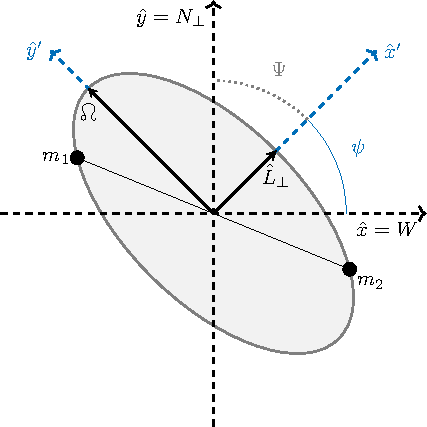
\includegraphics[width=0.8\columnwidth]{diagram_skyview.pdf}
\caption{View of Fig.~\ref{fig:diagram_sourceframe} as seen by the observer, with the LIGO-Virgo convention that $\Omega=\pi/2$. The masses rotate counterclockwise in the plane of the sky, spanned by the local west ($W$) and the in-sky projection of the celestial north ($N_\perp$).
}
\label{fig:diagram_skyview}
\end{figure}

In fact, with these conventions for a nonprecessing binary, the three angles $\psi$, $\Psi$ and $\theta$ can all be subsumed by a single parameter (usually written $\psi$) simultaneously encoding the orientation of our polarization basis, the alignment of the source in the sky, and the principal axes of the GW polarization ellipse.
We can then think of this angle as a property of the source to be measured from our data, rather than an arbitrary parameter orienting our frame.
Although this equivocation vastly simplifies analyses, it is helpful to keep in mind that the three angles are conceptually distinct: $\psi$ can always be defined, but $\theta$ only exists for fully polarized waves, and $\Omega$ is an orbital element, not defined for arbitrary sources (say, a stochastic source, or a supernova).

If the component spins are not (anti)aligned with the orbital angular momentum, the spins and the orbital plane will both precess.
As a consequence, the system will not be reflection symmetric and the GW signal will not be elliptically polarized overall.
Nonetheless, it is still conventional to tie $\hat{y}$ to the source as in Fig.~\ref{fig:diagram_sourceframe}, referring to the line of nodes as oriented at some specific point in the binary evolution (e.g., when the detected GW signal reaches 20 Hz).

In summary, we can identify three conceptually distinct Cartesian frames: a wave frame that determines the principal directions along which we \emph{define} the effect of a plus vs cross wave; for an elliptical wave, an intrinsic polarization frame, encoding the principal directions of the polarization ellipse; and a source frame, aligned with the symmetries of the source, or otherwise anchored to some defining feature of it; all of these can be specified in some astronomical frame, like ecliptic celestial coordinates.
For nonprecessing binaries, which are highly symmetric, we can define the source frame to make it always align with the polarization frame.

In unmodeled analyses, as those discussed in Sec.~\ref{sec:ellip:gen}, it is not possible or useful to explicitly tie the polarization frame to properties of the source, since these analyses are not tailored to any specific source to begin with, or they purposely disregard source orientation information for the sake of generality.
In that case, the model for $h_+$ and $h_\times$ can be defined in any arbitrary wave frame.
A common choice is to simply set $\psi = 0$ in the standard coordinates described above, i.e., with $\hat{y}$ pointing towards the celestial north (Fig.~\ref{fig:diagram_sourceframe}).
Having done so, all information regarding polarization orientation will be encoded in the $\theta$ parameter of Fig.~\ref{fig:ellipse}, with one value per elliptical mode in the decomposition of \eq{ellip_sum}.
Varying both $\psi$ and $\theta$ simultaneously is ill-advised in that context, since the two parameters will be fully degenerate (see end of Sec.~\ref{sec:ellip}).

\section{Coordinate transformations}

In the previous sections, we have introduced different parametrizations of elliptical (fully polarized) waves, including Eqs.~\eqref{eq:ellip_circ}, \eqref{eq:hcomp_ellip} and \eqref{eq:hcomp_ellip_chi}.
Their use varies depending on the specific application, according to convenience and convention.
Understanding the relation between the different parametrization becomes especially important when implementing and interpreting measurements, since the choice of parametrization influences the prior specified in the analysis.
Measurements obtained with different parametrizations may be related via a Jacobian.

We may also want to switch parametrizations for technical reasons.
Although conceptually insightful, the manifestly-elliptical parameterization in terms of $\{A, \epsilon, \theta, \phi\}$ of \eq{hcomp_ellip} contains multiple degeneracies that make it less than ideal for sampling purposes.
For instance, the angles $\theta$ and $\phi$ become totally degenerate when $\epsilon = \pm 1$; another degeneracy appears as $\theta \to \theta + \pi$ and $\epsilon \to - \epsilon$.
To circumvent this, we may switch to a more suitable parametrization in the sampling process, and then translate the result back into $\{A, \epsilon, \theta, \phi\}$ for interpretation.
In that case, we can still specify a prior in terms of the elliptical quantities by again making use of a Jacobian.

\begin{figure}
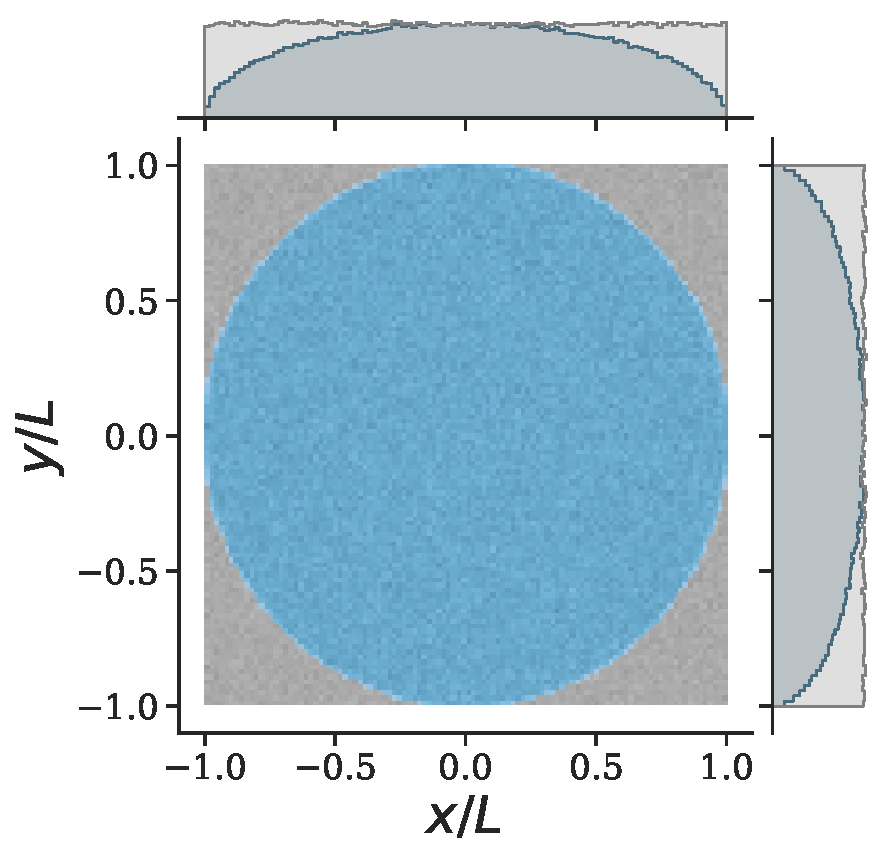
\includegraphics[width=0.49\columnwidth]{jac_example_0}
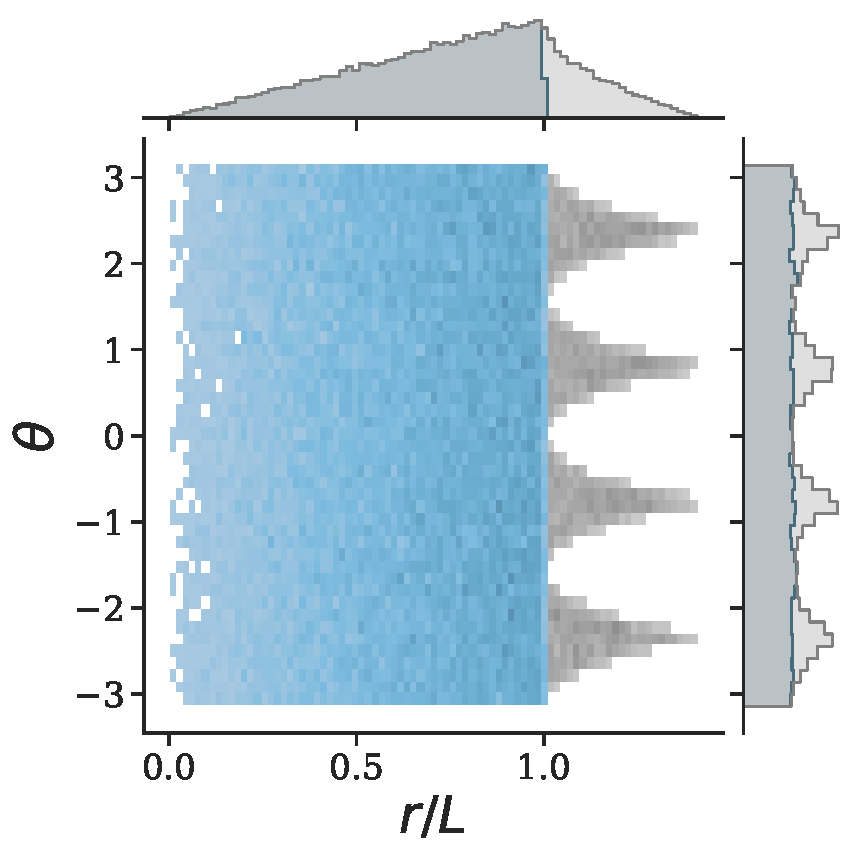
\includegraphics[width=0.49\columnwidth]{jac_example_1}
\caption{Example of coordinate transformations for probability distributions.
Sampling uniformly in some Cartesian coordinates $-L \leq x \leq L$ and $-L \leq y \leq L$ (gray left), where $L$ is some arbitrary scale, imposes a nonuniform distribution in the corresponding polar coordinates $r = \sqrt{x^2 + y^2}$ and $\theta = \arctan(y/x)$ (gray right); we obtain a more restricted distribution if we limit the sampling to a disk $x^2 + y^2 < L^2$ instead of a square (blue). 
Up to $r < L$ the density is uniform in $\theta$ and proportional to $r$ (top right), while for $r>L$ there are spikes of probability at $\theta = \pm \pi/4,\pm 3\pi/4$ (right side), corresponding to the corners of the square on the left.
We can recover a uniform distribution in $(r, \theta)$ by applying a Jacobian $\propto 1/r$ per \eq{jac}, and explicitly restricting to $r< L$ (blue), thus cutting out the corners of the left-hand square.}
\label{fig:jac_example}
\end{figure}

If we parametrize our analysis in terms of some alternative set of parameters $\vec{\xi}$, we can impose some prior distribution defined in the space of elliptical quantities, $p({A, \epsilon, \theta, \phi})$, by choosing a corresponding prior $p(\vec{\xi})$ for the $\vec{\xi}$ quantities such that
\begin{equation} \label{eq:jac}
p \left( \vec{\xi} \right) = p \left( A, \epsilon, \theta, \phi \right) \left| \frac{\partial \{A, \epsilon, \theta, \phi\}}{\partial \vec{\xi}} \right| ,
\end{equation}
where the last factor $J \equiv | \partial (A, \epsilon, \theta, \phi)/\partial \vec{\xi} |$ is the determinant of the Jacobian matrix.
Applying the Jacobian without any further reweighting yields a flat prior on the  $\{A, \epsilon, \theta, \phi\}$ quantities over the region covered by the original prior.
As with any coordinate transformation, the integration limits must be adjusted to ensure that they correspond to the targeted region in the $\{A, \epsilon, \theta, \phi\}$ space---for example, sampling uniformly in the two Cartesian quadratures $(x, y)$, we can effect a uniform prior on the polar quantities $(0 < r=\sqrt{x^2+y^2} \leq L, \theta= \arctan y/x)$ by applying a Jacobian $\propto 1/r$ and explicitly enforcing $r \leq L$ (Fig.~\ref{fig:jac_example}).

In this section, we will consider four different parametrizations of an elliptical wave, and present the Jacobians relating them to the $\{A, \epsilon, \theta, \phi\}$ parametrization.
We will focus on a single elliptical component as a standin for any individual term in the sum of Eq.~\eqref{eq:ellip_sum}, so that the results are trivially generalizable to decompositions of GWs with arbitrary polarizations, as would be used by \textsc{BayesWave} or other generic analyses.
We assume the amplitude could potentially subsume any (slow) time dependence present implied by $\mathcal{A}(t)$ in Eq.~\eqref{eq:ellip_gen}, e.g., the amplitude parameters below could correspond to a reference amplitude $A=\mathcal{A}(t=0)$.

\subsection{Amplitude and ellipticity}
\label{sec:jac:Achi}

\begin{figure}
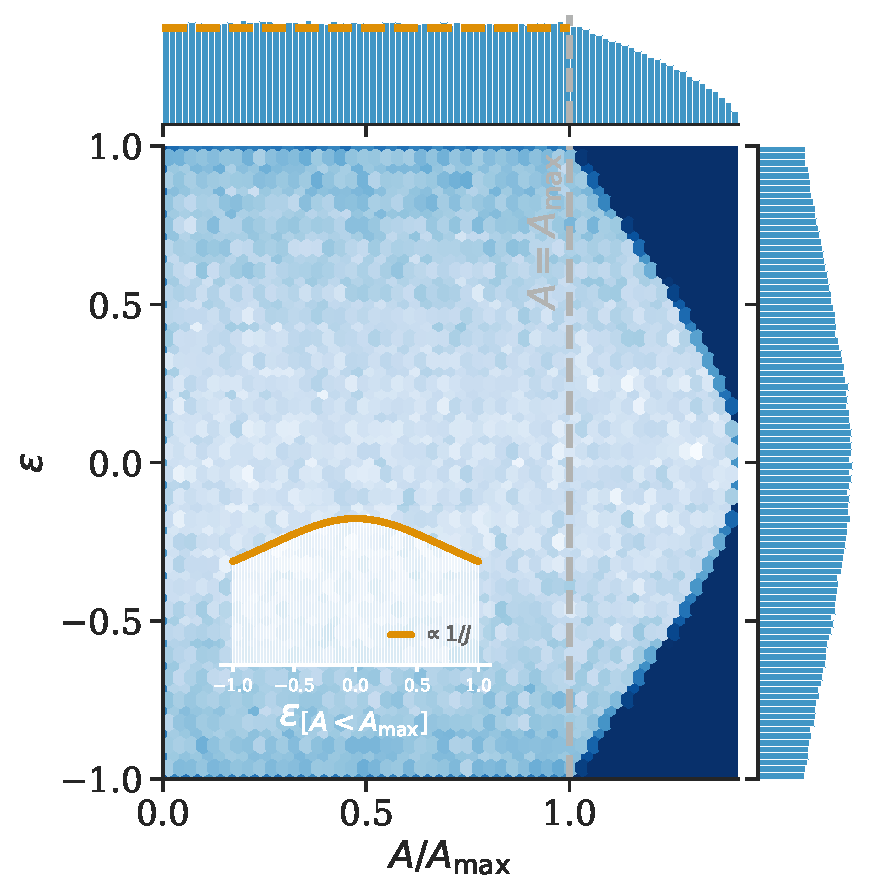
\includegraphics[width=0.8\columnwidth]{jac_Aeps_Achi}
\caption{Distribution imposed on $\{A,\epsilon\}$ by applying a flat prior on $\{\hat{A},\chi\}$ over the ranges $0 < \hat{A} \leq \hat{A}_{\max}$ and $-\pi/4 \leq \chi \leq \pi/4$.
Since $\hat{A} = A \sqrt{1+\epsilon^2}$ and $\max(\epsilon)= 1$, we should make sure to bound $A \leq  A_{\max} \equiv \hat{A}_{\max} /\sqrt{2}$ (dotted line), as in the example of Fig.~\ref{fig:jac_example}.
With that constraint (blue), the $A,\epsilon$ distribution is inversely proportional to the Jacobian in \eq{jac_Aeps_Achi}: a uniform prior on $\hat{A}$ and $\chi$ is uniform in $A$ but slightly favors linear polarizations ($\epsilon = 0$) over circular ones ($\epsilon = \pm 1$), with probability density $\propto 1/J_0$ (dashed curves). 
The marginal histograms are normalized by bin count.
}
\label{fig:jac_Aeps_Achi}
\end{figure}

In Sec.~\ref{sec:ellip:mono}, we presented two equivalent parametrizations of the $h_{+/\times}$ components of an elliptical wave, Eqs.~\eqref{eq:hcomp_ellip} and \eqref{eq:hcomp_ellip_chi}, illustrated in Fig.~\ref{fig:ellipse}.
Equation ~\eqref{eq:hcomp_ellip} parametrizes the signal strength via the maximum amplitude achieved by the wave, $A$ (the semimajor axis in Fig.~\ref{fig:ellipse}), and the shape of the polarization ellipse via the ellipticity, $\epsilon$ (the ratio between the semiminor and semimajor axes);
meanwhile, Eq.~\eqref{eq:hcomp_ellip_chi} parametrizes the strength via the intensity amplitude $\hat{A}$, which is the square-root of the signal intensity $I$, and the shape of the ellipse throught the angle $\chi$.
The two parametrizations are straigthforwardly related by
\begin{equation} \label{eq:Aellip_Ahatchi}
\begin{cases}
\hat{A} = A \sqrt{1 + \epsilon^2} \\
\chi = \arctan \epsilon 
\end{cases} 
\end{equation}
and the inverse transformation
\begin{equation} \label{eq:Ahatchi_Aellip}
\begin{cases}
A = \hat{A} \cos \chi \\
\epsilon = \tan \chi \\
\end{cases} ,
\end{equation}
with no change to the angles $\theta$ and $\phi$.
The Jacobian relating these two transformations is simply
\begin{equation} \label{eq:jac_Aeps_Achi}
J_0 \equiv \left| \frac{\partial(A,\epsilon,\theta,\phi)}{\partial(\hat{A}, \chi, \theta, \phi)}\right| =  \sec \chi = \sqrt{1 + \epsilon^2} \, ,
\end{equation}
or, equivalently $J_0 = \hat{A}/A$.
This Jacobian, illustrated in Fig.~\ref{fig:jac_Aeps_Achi}, indicates that a uniform prior in the $\{\hat{A}, \chi\}$ quantities implicitly favors linear polarizations relative to circular ones.

\subsection{Circular components}
\label{sec:jac:Arl}

An monochromatic elliptical wave, Eq.~\eqref{eq:hcomp_ellip}, can be specified in terms of the circular polarization basis elements as in \eq{ellip_circ},
where the $C_{R/L} \equiv A_{R/L} \exp(i\phi_{R/L})$ quantities control the amplitude and phase of the right and left circularly-polarized components of the signal.
%
The representation in terms of such circular-mode amplitudes and phases is equivalent to Eq.~\eqref{eq:hcomp_ellip} if we impose
\begin{equation} \label{eq:Cphi_to_Aellip}
\begin{cases}
A = \frac{1}{\sqrt{2}}\left(A_R + A_L\right) \\
\epsilon = (A_R - A_L)/(A_R + A_L) \\ 
\theta = \frac{1}{2}(\phi_L - \phi_R)\\
\phi = \frac{1}{2}(\phi_L + \phi_R)\\
\end{cases} .
\end{equation}
Equivalently, the inverse transformation is 
\begin{equation} \label{eq:Aellip_to_Cphi}
\begin{cases}
A_R = \frac{1}{\sqrt{2}} A \left(1 + \epsilon\right) \\
A_L = \frac{1}{\sqrt{2}} A \left(1 - \epsilon\right) \\
\phi_R = \phi - \theta \\ 
\phi_L = \phi + \theta \\ 
\end{cases} .
\end{equation}
These expressions are particularly simple: amplitude parameters $\{ A_R, A_L\}$ transform directly into amplitude parameters $\{A, \epsilon\}$, irrespective of phasing angles.
This is a consequence of the fact that the circular polarizations are defined to be invariant under rotations around the direction of propagation, up to an overall phase as shown in \eq{htransf_circ}.

The above transformations imply a Jacobian
\begin{equation} \label{eq:jac_Aeps_Arl}
J_1 \equiv \left| \frac{\partial(A,\epsilon,\theta,\phi)}{\partial(A_R, A_L, \phi_R, \phi_L)}\right| \propto \frac{1}{A_R + A_L}\, ,
\end{equation}
with a proportionality constant of $1/\sqrt{2}$, which is ignored in most applications as it can be absorbed by an overall normalization; based on \eq{Cphi_to_Aellip}, this is also proportional to $1/A$.
Therefore, a prior uniform in $A_R$ and $A_L$ results in a triangular prior in the overall amplitude of the mode defined by $A$ (Fig.~\ref{fig:jac_Aeps_Arl}).
An isotropic prior in $0 < \phi_{R/L} < 2\pi$ is also uniform in $0 < \theta <\pi$ and $0 < \phi <\pi$.

Equation \eqref{eq:jac_Aeps_Arl} implies that an analysis that samples uniformly in $A_R$ and $A_L$ within some range $0 \leq A_{R,L} \leq A_{R/L,\mathrm{max}}$ actually favors large overall mode amplitudes $A$, with a triangular distribution that vanishes at $A=0$ and $A=\sqrt{2}\,A_{R/L,\mathrm{max}}$, and peaks at $A = A_{R/L,\mathrm{max}}/\sqrt{2} \equiv A_{\max}$ (top panel of Fig.~\ref{fig:jac_Aeps_Arl}).
Without enforcing a $A \leq A_{\max}$ constraint, the ellipticity distribution will no longer be uniform, instead favoring linear polarizations (left panel of Fig.~\ref{fig:jac_Aeps_Arl}).
This was the case, e.g., for one of the ringdown analyses in \cite{LIGOScientific:2020tif}, which sampled uniformly in amplitude coefficients equivalent to $A_{R/L}$ up to an overall scaling.

\begin{figure}
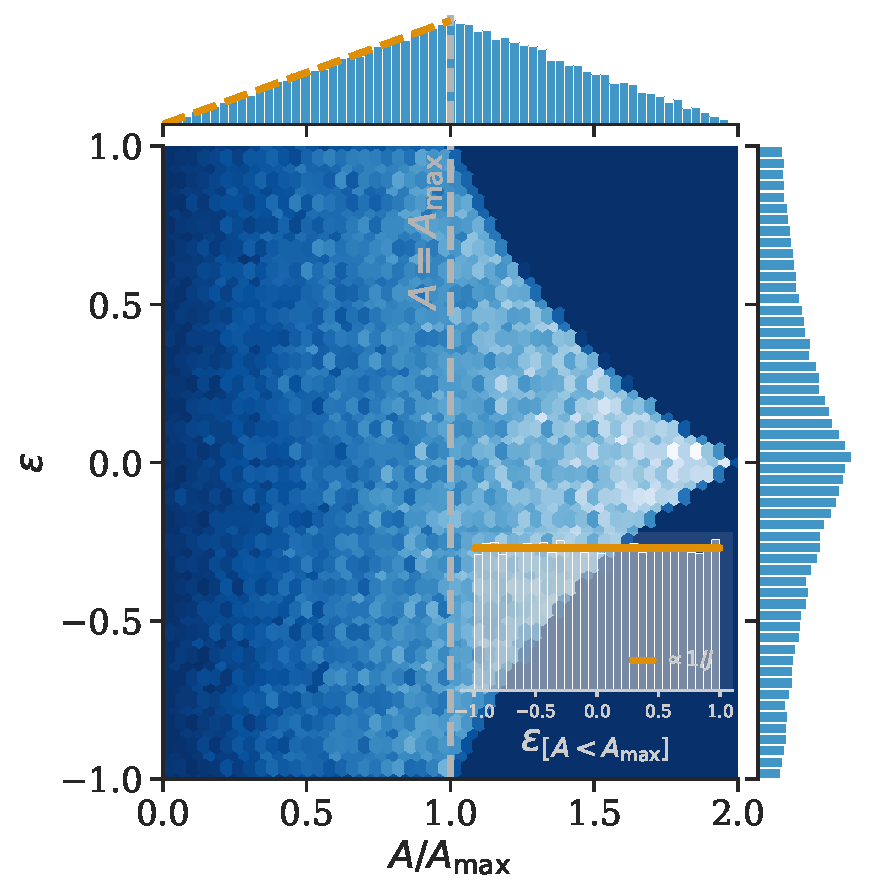
\includegraphics[width=0.8\columnwidth]{jac_Aeps_Arl}
\caption{Distribution imposed on $\{A,\epsilon\}$ by applying a flat prior on $\{A_R,A_L\}$ over the ranges $0 < A_{R/L} \leq A_{R/L,\max}$.
Since $A = (A_R + A_L)/\sqrt{2}$, we must constrain $A \leq A_{\max} \equiv A_{R/L,\max}/\sqrt{2}$ (dotted line), as in the example of Fig.~\ref{fig:jac_example};
failing to do so would result in a triangular distribution for $A$, i.e., upward sloping for $A < A_{\max}$ and downward sloping for $A > A_{\max}$ (top panel), and a nonunform distribution on $\epsilon$ (right panel).
Restricting to $A < A_{\max}$ (blue), the density is proportional to $A$ and flat in $\epsilon$, following $\propto 1/J_1$ for the Jacobian in \eq{jac_Aeps_Arl} (dashed curves).
The marginal histograms are normalized by bin count.
}
\label{fig:jac_Aeps_Arl}
\end{figure}

We can also relate the circular amplitudes to the alternative parametrization of \eq{hcomp_ellip_chi}.
The straightforward relation is given by the transformations
\begin{equation} \label{eq:Cphi_to_Ahatchi}
\begin{cases}
\hat{A} = \sqrt{A_R^2 + A_L^2} \\
\chi = \arctan\left( \frac{A_R - A_L}{A_R + A_L}\right)
\end{cases} ,
\end{equation}
and
\begin{equation} \label{eq:Cphi_to_Ahatchi}
\begin{cases}
A_R = \frac{1}{\sqrt{2}} \hat{A} \left(\cos\chi + \sin \chi\right) \\
A_L = \frac{1}{\sqrt{2}} \hat{A} \left(\cos\chi - \sin \chi\right)
\end{cases} ,
\end{equation}
while the remaining angles are related as in Eqs.~\eqref{eq:Cphi_to_Aellip} and \eqref{eq:Aellip_to_Cphi}.
Accordingly, the Jacobian that takes us from the circular parametrization to one flat in $\{\hat{A},\chi\}$ can be shown to be $J \propto \hat{A}^{-1}$.
Thus, as expected from the composition of Eqs.~\eqref{eq:jac_Aeps_Achi} and \eqref{eq:jac_Aeps_Arl}, a prior uniform in $A_{R/L}$ will also favor large intensity amplitudes with probability $\propto \hat{A}$, when restricted to the appropriate range; it will also be uniform in $\chi$.


\subsection{Linear components}
\label{sec:jac:Apc}

Rather than using the circular basis, we could instead work with the linear polarization modes as the fundamental quantity, parametrizing them directly as
\begin{subequations} \label{eq:Aphi}
\begin{equation}
h_+ = A_+ \cos (\omega t - \phi_+)\, ,
\end{equation}
\begin{equation}
h_\times = A_\times \cos (\omega t - \phi_\times) \, ,
\end{equation}
\end{subequations}
where $A_{+/\times}$ and $\phi_{+\times}$ are initial amplitudes and phases for each polarization, as elsewhere in the text.
Structurally, this mimics the parametrization adopted by \textsc{BayesWave} for each wavelet \cite{Cornish:2020dwh}.

\newcommand{\xp}{x_{+}}
\newcommand{\xc}{x_{\times}}
\newcommand{\xpc}{x_{+/\times}}
\newcommand{\yp}{y_{+}}
\newcommand{\yc}{y_{\times}}
\newcommand{\ypc}{y_{+/\times}}

\newcommand{\xr}{x_{R}}
\newcommand{\xl}{x_{L}}
\newcommand{\xrl}{x_{R/L}}
\newcommand{\yr}{y_{R}}
\newcommand{\yl}{y_{L}}
\newcommand{\yrl}{y_{R/L}}

% \newcommand{\xp}{A_{+,c}}
% \newcommand{\xc}{A_{\times,c}}
% \newcommand{\xpc}{A_{+/\times,c}}
% \newcommand{\yp}{A_{+,s}}
% \newcommand{\yc}{A_{\times,s}}
% \newcommand{\ypc}{A_{+/\times,s}}

\begin{figure}
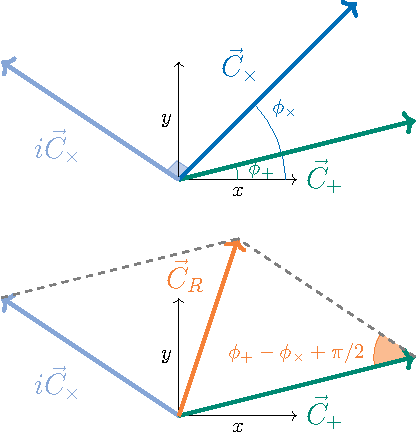
\includegraphics[width=\columnwidth]{diagram_apac}
\caption{Geometric derivation of Eq.~\eqref{eq:Aphi_to_Cphi} for the left-handed polarization case.
\emph{Left:} Following Eq.~\eqref{eq:Aphi}, the plus and cross Jones-vecor amplitudes, $\vec{C}_{+/\times} = A_{+/\times} \exp(i \phi_{+/\times})$, subtend angles $\phi_{+/\times}$ relative to the real axis ($x$, abscissa) and thus have Cartesian coordinates $\left(\xpc, \ypc \right)$, in terms of the quadratures defined in Eq.~\eqref{eq:xy}; the vector $i\vec{C}_\times$ is orthogonal to $\vec{C}_\times$, so that it subtends an angle $\pi/2 + \phi_\times-\phi_+$ with respect to $\vec{C}_+$.
\emph{Right:} the left-handed Jones amplitude, $\vec{C}_L = (\vec{C}_+ + i \vec{C}_\times)/\sqrt{2}$, has components $\left(\xp - \yc, \yp + \xc\right)/\sqrt{2}$ and, therefore, $\phi_R = \mathrm{atan2}( \yp + \xc, \xp - \yc)$; since the acute angle between $\vec{C}_+$ and $i\vec{C}_\times$ is $\pi - (\pi /2 + \phi_\times - \phi_+) = \phi_+ - \phi_\times + \pi/2$, the law of cosines Eq.~\eqref{eq:Aphi_to_Cphi} for $A_L$. (The right-handed case is analogous).
}
\label{fig:diagram_apac}
\end{figure}

Equation \eqref{eq:Aphi} still represents an elliptically polarized mode.
To relate this parametrization to that in Eq.~\eqref{eq:hcomp_ellip}, it is convenient to first map Eq.~\eqref{eq:Aphi} into the circular-basis parameters of the previous section.
We can do this geometrically by considering the respective Jones vectors (Sec.~\ref{sec:math}), from which we get $C_{R/L} = (C_+ \mp i C_\times)/\sqrt{2}$, for $C_{+/\times} \equiv A_{+/\times} \exp(i\phi_{+/\times})$ as in \eq{jones_bases}.
As illustrated in Fig.~\ref{fig:diagram_apac}, trigonometry then implies that
\begin{equation} \label{eq:Aphi_to_Cphi}
\begin{cases}
A_R^2 = \frac{1}{2}\left[A_+^2 + A_\times^2 + 2 A_+ A_\times \sin(\phi_\times - \phi_+)\right] \\
A_L^2 = \frac{1}{2}\left[A_+^2 + A_\times^2 - 2 A_+ A_\times \sin(\phi_\times - \phi_+)\right] \\
\phi_R = \mathrm{atan2}\left(\yp -\xc, \xp + \yc \right)\\
\phi_L = \mathrm{atan2}\left(\yp + \xc, \xp - \yc \right) 
\end{cases} ,
\end{equation}
where, to simplify the notation, we have defined the cosine and sine quadratures
\begin{subequations} \label{eq:xy}
\begin{equation}
\xpc \equiv A_{+/\times} \cos \phi_{+/\times} \, ,
\end{equation}
\begin{equation}
\ypc \equiv A_{+/\times} \sin \phi_{+/\times} \, .
\end{equation}
\end{subequations}
Together with Eq.~\eqref{eq:Cphi_to_Aellip}, this allows us to compute $\{A, \epsilon, \theta, \phi\}$ as a function of $\{A_+, A_\times, \phi_+, \phi_\times\}$.
This transformation is clearly less straightforward than those for the circular components in the previous section, with amplitude and phase parameters mixing into each other.
This is because this coordinate transformation encodes the frame rotation that would bring an arbitrarily-oriented elliptical wave into the simple form of Eq.~\eqref{eq:Aphi}, which is nothing but the special frame we identified in Eq.~\eqref{eq:ellip_frame}.

The overall Jacobian relating $\{A, \epsilon, \theta, \phi\}$ to $\{A_+, A_\times, \phi_+, \phi_\times\}$ is quite simple, however, when expressed in terms of the former set of parameters,
\begin{subequations} \label{eq:jac_Aphi}
\begin{align}
J_2 &\equiv \left| \frac{\partial(A, \epsilon, \theta, \phi)}{\partial(A_+, A_\times, \phi_+, \phi_\times)}\right| \nonumber \\
&= 2 A_+ A_\times \left[ \sqrt{A_+^4 + A_\times^4 + 2 A_+^2 A_\times^2 \cos 2(\phi_\times - \phi_+)} \right. \nonumber \\
& \times \left( \sqrt{A_+^2 + A_\times^2 -2 A_+ A_\times \sin(\phi_\times-\phi_+)} \right. \nonumber \\
&\left.\left. +  \sqrt{A_+^2 + A_\times^2 +2 A_+ A_\times \sin(\phi_\times-\phi_+)}\right)\right]^{-1}\\
&= \frac{1}{2 A} \sqrt{\left(\frac{1 + \epsilon^2}{1 - \epsilon^2}\right)^2 - \cos^2 2\theta} \, .
\end{align}
\end{subequations}
The Jacobian factorizes into a piece for the size of the ellipse ($1/A$), and a less trivial piece for its shape and orientation (function of $\epsilon$ and $\theta$).
The $J_2 \propto 1/A$ dependence implies that an analysis with uniform priors in the linear polarization amplitudes will implicitly favor high overall signal power, as was the case for the circular amplitudes in Fig.~\ref{fig:jac_Aeps_Arl}.
Additionally, the dependence on the ellipse's shape implies that the Jacobian diverges to positive infinity for $\epsilon = \pm 1$, meaning that circular polarizations will be disfavored in this scenario.

\begin{figure}
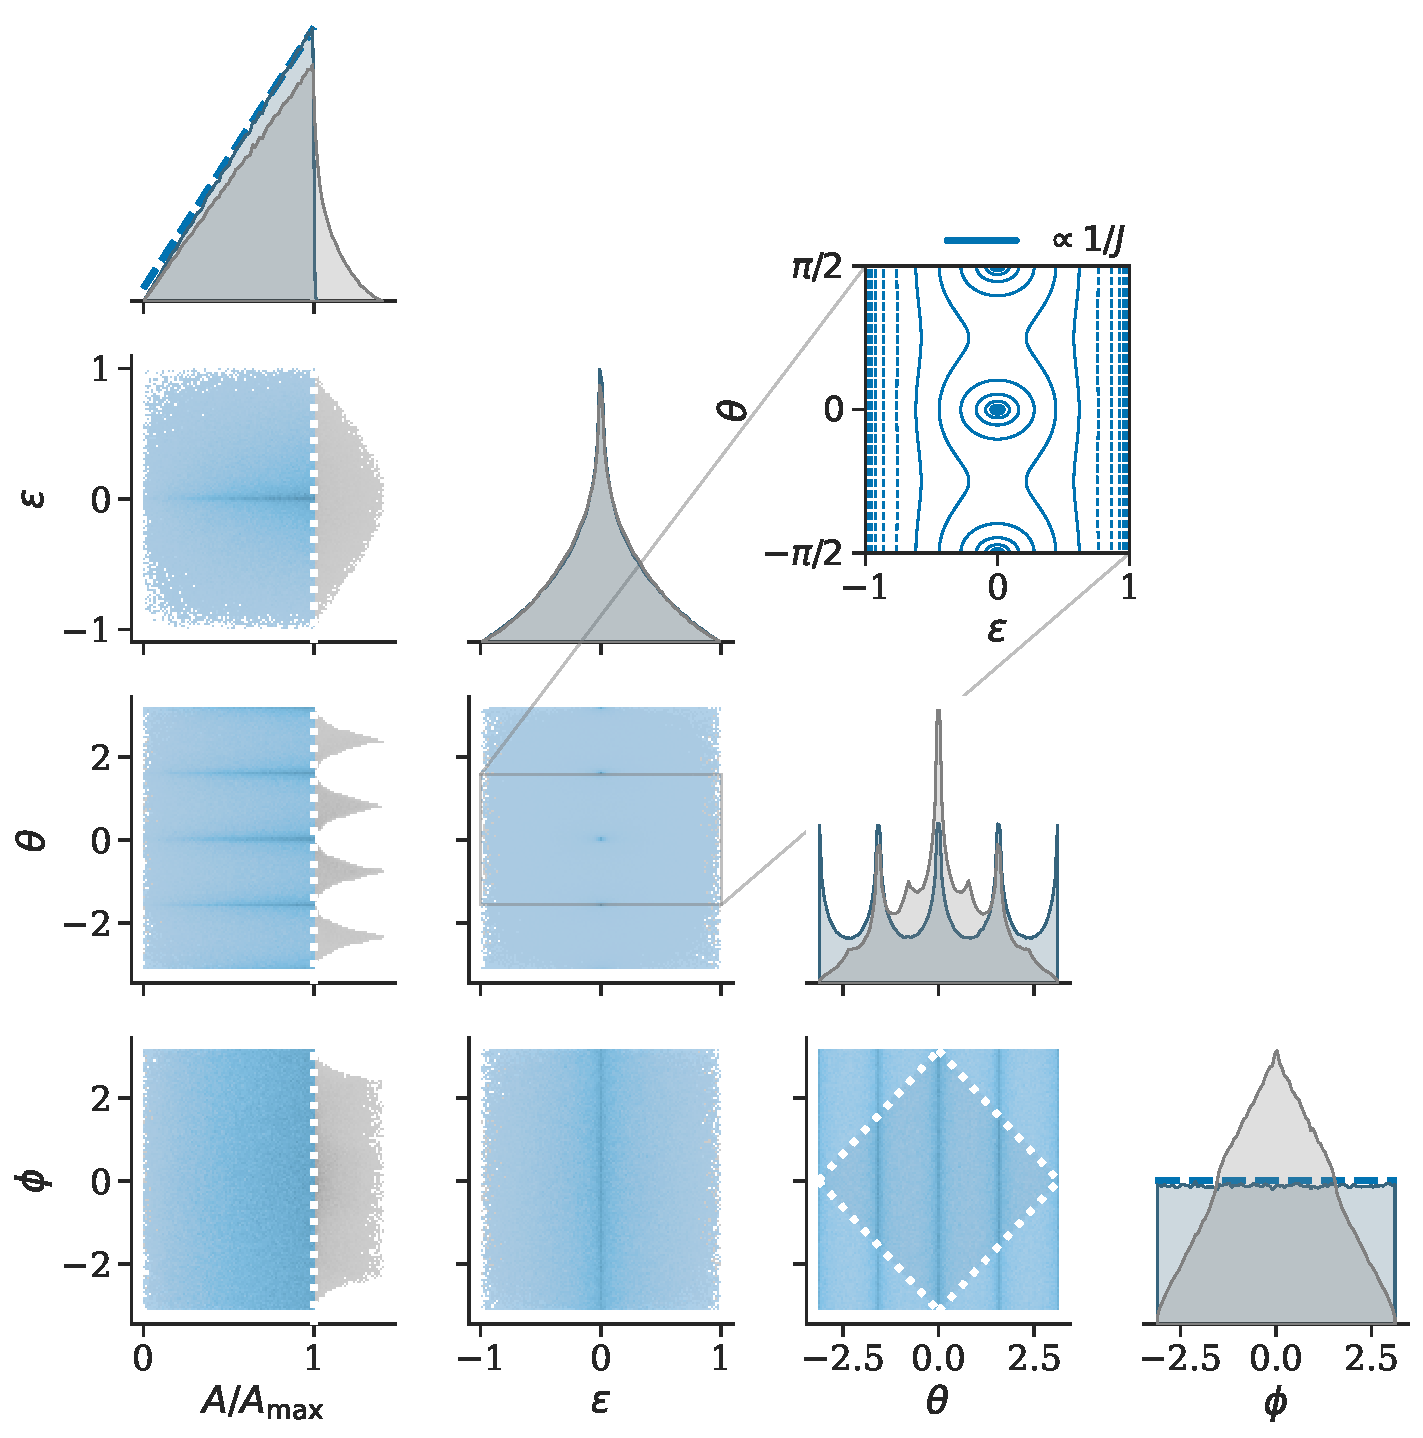
\includegraphics[width=\columnwidth]{jac_Aeps_Apc_corner}
\caption{Distribution imposed on $\{A,\epsilon, \theta, \phi\}$ by applying a flat prior on $\{A_+,A_\times, \phi_+, \phi_\times\}$, as defined in \eq{Aphi}, over the ranges $0 < A_{+/\times} \leq A_{\max}$ and $0 < \phi_{+/\times} < 2\pi$.
The blue distribution restricts parameters to the targeted range $0 < A < A_{\max}$, and $\pi/2 \leq \theta,\phi <\pi/2$, as in the example of Fig.~\ref{fig:jac_example}.
The 4D density is inversely proportional to the $J_2$ Jacobian in \eq{jac_Aphi}, which is represented by blue lines (over the marginals for $A$ and $\phi$, and in the inset for $\epsilon$ and $\theta$); in particular, the inset shows logarithmically-spaced contours of the $(\epsilon,\theta)$-dependent piece of $1/J_2$.
The difference between the blue and gray distributions for $\theta$ and $\phi$ is an artifact of the chosen angle ranges: it would not have appeared had we instead worked with $\bar{\theta} \equiv 2\theta$ and $\bar{\phi} \equiv 2\phi$, both in the range $[0,2\pi]$.
The marginal histograms are normalized by bin count.
The distribution represented here heavily favors linear polarizations ($\epsilon = 0$) along the $+/\times$ directions defined by \eq{Aphi} ($\theta = 0, \pm\pi/2$).
}
\label{fig:jac_Aphi}
\end{figure}

Both those features are visible in Fig.~\ref{fig:jac_Aphi}, which shows the distribution imposed on all of our canonical parameters, $\{A,\epsilon, \theta, \phi\}$, by drawing uniformly in $0 < A_{+/\times} < A_{\max}$ and $0 < \phi_{+/\times} < 2\pi$, for some arbitrary scale $A_{\rm max}$.
The distribution increases proportionally with $A$ up to $A_{\max}$ and peaks strongly at $\epsilon = 0$, sharply favoring linear polarizations.
In fact, the $\theta$ dependence of \eq{jac_Aphi} implies that pure $+$ or $\times$ polarizations ($\theta=0$ or $\theta = \pm\pi/2$, respectively) will be favored over any other orientation, i.e., pure linear polarizations aligned with the frame used to define $+$ and $\times$ in \eq{Aphi}.

The sharpness of the $\epsilon$ and $\theta$ features in Fig.~\ref{fig:jac_Aphi} suggests that fully correcting for the Jacobian in \eq{jac_Aphi} will be challenging in sampling applications.
Therefore, the parametrization of \eq{Aphi} is likely nonperformant if the goal is to obtain results under a uniform prior in $\{A,\epsilon\}$---we found this to be the case in practice in the context of \cite{Chatziioannou:2021mij}.
The parameterization is otherwise also likely undesirable if there is no known orientation of the polarization frame to favor in writing down \eq{Aphi}, i.e., in the language of Sec.~\ref{sec:angles}, if there is no a priori preferred polarization angle $\psi$.

\subsection{Linear polarization quadratures}
\label{sec:jac:Axy}

In the previous section we introduced the linear polarization quadratures $\xpc \equiv A_{+/\times} \cos \phi_{+/\times}$ and $\ypc \equiv A_{+/\times} \sin \phi_{+/\times}$, \eq{xy}, which are the Cartesian components (real and imaginary) corresponding to the complex-valued Jones amplitudes that encode the polarization state of the signal (see Fig.~\ref{fig:diagram_apac} and Sec.~\ref{sec:math}).
In \eq{Aphi_to_Cphi} we used these quantities to conveniently express the relation between the phases of the linear components of \eq{Aphi} and those of their circular counterparts, \eq{ellip_circ}, but their usefulness extends more widely.
Notably, the quadratures are usually more suitable for sampling applications, since working with periodic phases like $\phi_{+/\times}$ can be problematic for stochastic algorithms like Markov chain Monte Carlo (MCMC) \cite{Hogg:2017akh}.
Together with Gaussian priors, they can also make some problems analytically integrable \cite{Hogg:2020jwh}.

The usefulness of the linear-polarization quadratures stems from the fact that, unlike phase parameters like $\phi_{+/\times}$, they enter the waveform linearly.
Concretely, the expression for an elliptical monochromatic mode in terms of these quantities is
\begin{subequations} \label{eq:Axy}
\begin{equation}
h_+ = \xp \cos \omega t + \yp \sin \omega t \, 
\end{equation}
\begin{equation}
h_\times = \xc \cos \omega t + \yc \sin \omega t \, .
\end{equation}
\end{subequations}
The relation of $\xpc$ and $\ypc$ to the linear polarizations of \eq{Aphi} is given directly by the definition in \eq{xy}; such relation implies a transformation into the circular-polarization parameters given by
\begin{equation} \label{eq:Cphi_to_Axy}
\begin{cases}
A_R^2 = \frac{1}{2}\left[\left(\yp - \xc\right)^2 + \left(\xp + \yc\right)^2\right] \\
A_R^2 = \frac{1}{2}\left[\left(\yp + \xc\right)^2 + \left(\xp - \yc\right)^2\right] \\
\phi_R = \mathrm{atan2}\left(\yp -\xc, \xp + \yc \right)\\
\phi_L = \mathrm{atan2}\left(\yp + \xc, \xp - \yc \right) 
\end{cases} ,
\end{equation}
where last two lines are the same as in \eq{Aphi_to_Cphi}.
The inverse transformation is, as one might expect from Fig.~\ref{fig:diagram_apac},
\begin{equation} \label{eq:Axy_to_Cphi}
\begin{cases}
\xp = \frac{1}{\sqrt{2}} \left( \xr + \xl \right)\\
\yp = \frac{1}{\sqrt{2}} \left( \yr + \yl \right)\\
\xc = \frac{1}{\sqrt{2}} \left( \yl - \yr \right)\\
\yc = \frac{1}{\sqrt{2}} \left( \xr - \xl \right)\\
\end{cases} ,
\end{equation}
for circular-polarization quadratures defined as $\xrl \equiv A_{R/L}\cos\phi_{R/L}$ and $\yrl \equiv A_{R/L} \sin \phi_{R/L}$.

From \eq{Cphi_to_Aellip}, we can then derive a relation between $\{\xpc, \ypc\}$ and the canonical parameters $\{A,\epsilon,\theta,\phi\}$.
The inverse transformation, from  $\{A,\epsilon,\theta,\phi\}$ into $\{\xpc, \ypc\}$ is easier to express succinctly and is given by
\begin{equation} \label{eq:Axy_to_Cphi}
\begin{cases}
\xp = A \left(\cos\theta \cos\phi + \epsilon \sin\theta \sin\phi\right)\\
\yp = A \left(\cos\theta \sin\phi - \epsilon \sin\theta \cos\phi\right)\\
\xc = A \left(\sin\theta \cos\phi - \epsilon \cos\theta \sin\phi\right)\\
\yc = A \left(\sin\theta \sin\phi + \epsilon \cos\theta \cos\phi\right)
\end{cases} ,
\end{equation}
as is straightforward to check based on \eq{Axy} and \eq{hcomp_ellip} by basic trignometry.

The corresponding Jacobian is remarkably simple when expressed in terms of the ellipse amplitude and shape,
\begin{subequations} \label{eq:jac_Aeps_Axy}
\begin{align}
J_3 &\equiv 2 \left\{\sqrt{\left(\yp -\xc \right)^2 +\left(\xp +\yc\right)^2}
\right. \nonumber \\
&\times \sqrt{\left(\yp + \xc\right)^2 + \left(\xp - \yc\right)^2}  \nonumber\\
&\times \left[ \sqrt{\left(\yp -\xc \right)^2 +\left(\xp +\yc\right)^2} \right.  \nonumber\\
&+ \left.\left. \sqrt{\left(\yp + \xc\right)^2 + \left(\xp - \yc\right)^2} \right]\right\}^{-1} \\
&= \frac{1}{A^{3} \left(1 - \epsilon^2\right)}  .
\end{align}
\end{subequations}
This Jacobian again factorizes into a piece for the size of the polarization ellipse and another for its shape, but without a dependence on the ellipse orientation.
The scale-dependent factor ($1/A^3$) indicates that a flat prior on $\{\xpc,\ypc\}$ will strongly favor large signal amplitudes.
Like in \eq{jac_Aphi}, this $J_2$ diverges for $\epsilon = \pm 1$ which means that circular polarizations will be disfavored, albeit less strongly than $J_2$.
The lack of dependence of $J_3$ on the orientation ellipse $\theta$ indicates that no specific polarization frame is framed by this prior, reflecting the isotropy built into the definition of $\xpc, \ypc$.

The features described above are visible in the distribution imposed on $\{A,\epsilon,\theta,\phi\}$ by drawing uniformly on $\{\xpc, \ypc\}$, as shown in Fig.~\ref{fig:jac_Axy} for $A$ and $\epsilon$.
Over the targeted region ($A < A_{\max}$) the distribution steeply favors high signal amplitudes; it also favors linear polarizations ($\epsilon = 0$), although less sharply.
Enforcing $A < A_{\max}$, no specific value of $-\pi/2 < \theta, \phi < \pi/2$ is preferred; however, a similar structure to that in Fig.~\ref{fig:jac_Aphi} would appear outside that range of angles, which can again be mitigated by working with $\bar{\theta}$ and $\bar{\phi}$ instead.
The constraint on the amplitude, $A < A_{\rm max}$, is crucial to guarantee isotropy in the ellipse orientation: without it, the corners of the squares defined by $-A_{\max} < \xpc,\ypc < A_{\max}$ would result in special directions of high probability, just as in the example of Fig.~\ref{fig:jac_example}.
The same result could be obtained by applying an intrinsically isotropic prior in the $\{\xpc, \ypc\}$ space, e.g., uncorrelated Gaussians.

\begin{figure}
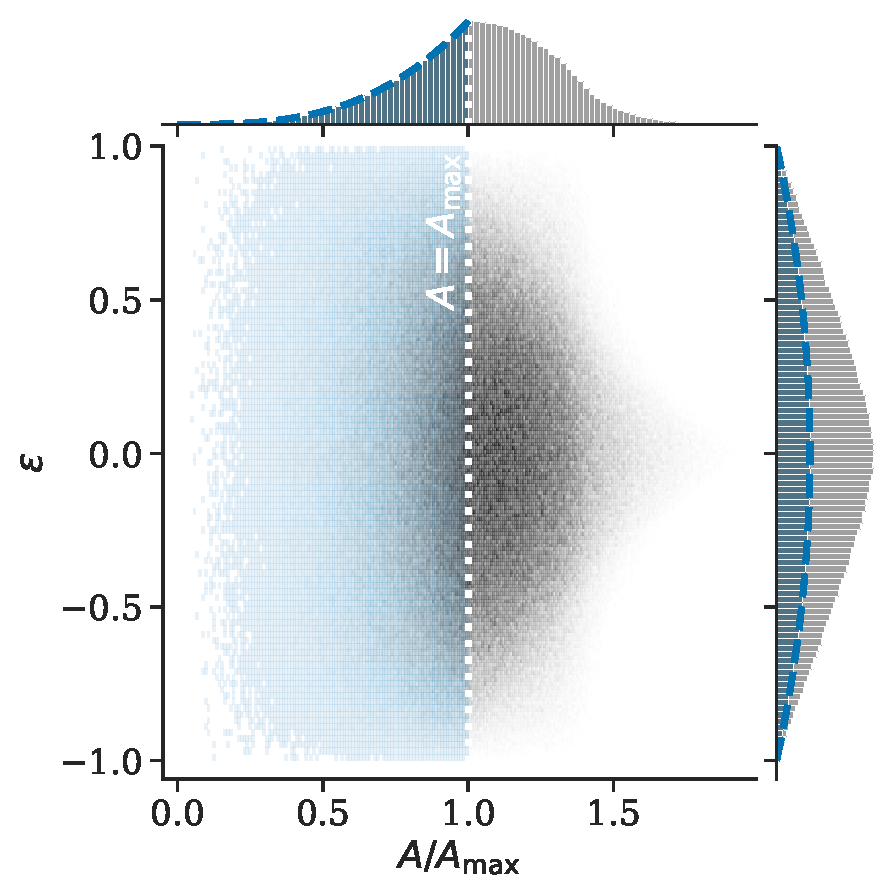
\includegraphics[width=\columnwidth]{jac_Aeps_Axy}
\caption{Distribution imposed on $\{A,\epsilon\}$ by applying a flat prior on $\{\xp, \yp, \xc, \yc\}$, as defined in \eq{xy}, over the ranges $- A_{\max} < \xpc,\ypc \leq A_{\max}$.
The blue distribution restricts the parameters to the targeted region, $A < A_{\max}$, as explained in the example of Fig.~\ref{fig:jac_example}.
Over that range, the probability density is inversely proportional to the Jacobian in \eq{jac_Aeps_Axy}: favoring large amplitudes and linear polarizations (dashed blue curves).
As in Fig.~\ref{fig:jac_Aphi}, the corresponding distribution over the angles $\theta$ and $\phi$ is isotropic when restricted to the appropriate range of $-\pi/2/ \leq \theta,\phi \leq \pi/2$ (not shown).
}
\label{fig:jac_Axy}
\end{figure}

\subsection{Inclination of a planar source}
\label{sec:jac:cosi}

There are several applications for which it is desirable to make a connection between the ellipticity of a signal and the corresponding inclination angle of a source via \eq{ellip_cosi}.
This is because even unmodeled analyses, like \textsc{BayesWave}, often target sources that are dominated by the quadrupolar harmonic of the radiation ($\ell=|m|=2$), and that can be presumed to respect the planar symmetry that gave rise to that equation (see Sec.~\ref{sec:harmonics}).

In that case, a physically meaningful prior for the shape of the polarization ellipse is usually one that is uniform in $\cos\iota$, corresponding to an isotropic prior on the source orientation.
Such a prior is necessarily nonuniform in $\epsilon$, as can be inferred from the relation between the two quantities, illustrated above in Fig.~\ref{fig:ellip_cosi}: uniform draws in $\cos\iota$ will necessarily favor circular polarizations over linear ones, since the $\epsilon$ versus $\cos\iota$ curve flattens at the edges as $\cos\iota\to\pm 1$ and $\epsilon \to \pm 1$.
Conversely, a prior uniform in $\epsilon$ will necessarily disfavor face on ($\cos\iota=+1$) or face off ($\cos\iota=-1$) sources.

Indeed, the Jacobian $J_4 \equiv \left|\partial\epsilon/\partial \cos\iota\right|$, transforming from $\cos\iota$ to $\epsilon$, is
\begin{equation} \label{eq:jac_eps_cosi}
J_4 =1 - \epsilon^2 + \sqrt{1-\epsilon^2} 
\propto \frac{1 - \cos^2\iota}{\left(1+\cos^2\iota\right)^2} \, ,
\end{equation}
which vanishes for $\cos\iota = \pm 1$ (or, equivalently, $\epsilon = \pm 1$) and peaks at $\cos\iota = 0$ ($\epsilon= 0$).
This indicates that a distribution uniform in $\cos\iota$ will place infinite weight on $\epsilon = \pm 1$, while a distribution uniform in $\epsilon$ will place no weight on $\cos\iota = \pm 1$ (left and right panels in Fig.~\ref{fig:jac_cosi}, respectively).

The divergences of the Jacobian above complicates transformations from one prior to the other, and suggest their implementation in sampling applications is likely nonperformant---in other words, if the goal is to apply a uniform prior on $\cos\iota$, then we should sample in that quantity directly, not $\epsilon$.

This issue becomes more pronounced if, rather than being uniform in $\epsilon$, the original prior itself disfavored $\epsilon = \pm 1$ in the first place.
This was the case for the parametrization in terms of $\hat{A}$ and $\chi$ in Sec.~\ref{sec:jac:Achi}, the linear polarization amplitudes in Sec.~\ref{sec:jac:Apc} and the linear polarization quadratures in Sec.~\ref{sec:jac:Axy}.
Of all these, the problem is most severe for the linear polarization amplitudes, since that parametrization places high weight (formally infinite) on $\epsilon = 0$ (Fig.~\ref{fig:jac_Aphi}).
Unfortunately, this was the parametrization used in \cite{Chatziioannou:2021mij}, which likely explains the difficulty in recovering the sky location of the circularly-polarized ($\cos\iota=1$) signal simulated in Fig.~11 of that work.

\begin{figure}
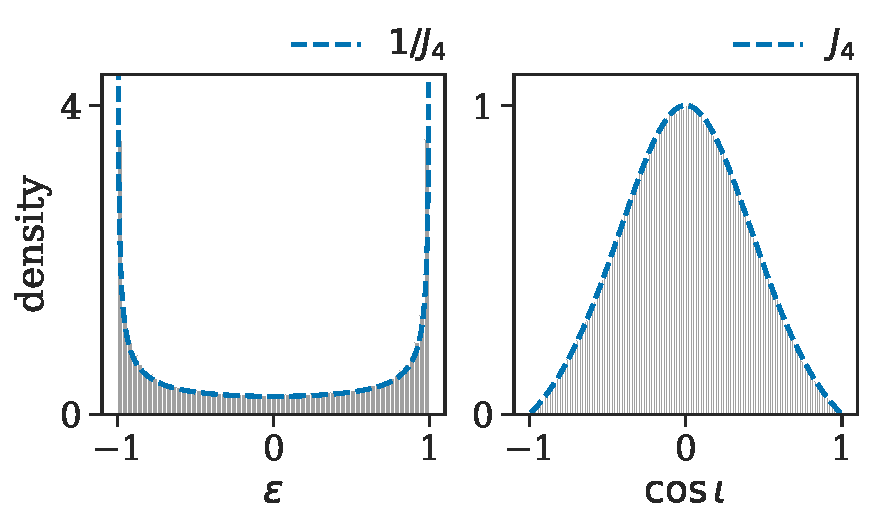
\includegraphics[width=\columnwidth]{jac_eps_cosi}
\caption{\emph{Left:} Probability density imposed on $\epsilon$ by applying a flat prior on $\cos\iota$, which is inversely proportional to the Jacobian $J_4$ in \eq{jac_eps_cosi}; this diverges at $\epsilon = \pm 1$.
\emph{Right:} Distribution imposed on $\cos\iota$ by a flat prior on $\epsilon$, which is directly proportional to \eq{jac_eps_cosi}; this vanishes at $\cos\iota = \pm 1$.
}
\label{fig:jac_cosi}
\end{figure}

\section{Nontensor polarizations}
\label{sec:nongr}

\newcommand{\xsym}{\ensuremath{\rm x}}
\newcommand{\ysym}{{\rm y}}
\newcommand{\bsym}{{\rm b}}
\newcommand{\lsym}{{\rm l}}
\newcommand{\hx}{h_{\xsym}}
\newcommand{\hy}{h_{\ysym}}
\newcommand{\hb}{h_{\bsym}}
\newcommand{\hlon}{h_{\lsym}}

Metric theories beyond GR may allow up to six independent polarizations, including the two tensor $+$ and $\times$ modes expected in GR.
The discussion above generalizes easily to include those additional modes, starting with an enhanced version of the driving matrix in Eq.~\eqref{eq:hij},
\beq \label{eq:hij_ngr}
(h_{ij}) = \begin{pmatrix}
\hb + h_+ & h_\times  & \hx  \\
h_\times  & \hb - h_+ & \hy  \\
\hx    & \hy    & \hlon
\end{pmatrix} ,
\eeq
where, in addition to plus and cross, also appear the vector-$x$ (\xsym) and vector-$y$ modes (\ysym), as well as the scalar breathing (\bsym) and longitudinal (\lsym) modes;%
\footnote{There are other possible normalizations in use in the literature, e.g., $\hlon \to \sqrt{2} \hlon$.}
Equivalently, as above, we can write this as a weighted sum over polarization tensors,
\beq
h_{ij} = \sum_p h_p\, e^p_{ij} \, ,
\eeq
for $p$ in $\{+,\times, \xsym, \ysym, \bsym, \lsym\}$, and polarization tensors $e^p_{ij}$ defined implicitly by comparison with Eq.~\eqref{eq:hij_ngr}.
Generally, the $h_p$ are functions of time, as for plus and cross above.
%
With similar assumptions as in the GR case, the detector output can be written as a sum over polarizations weighted by antenna patterns,
\beq \label{eq:h_ngr}
h(t) = \sum_p F_p(\alpha, \delta; \psi)\, h_p(t)\, ,
\eeq
with $F_p \equiv D^{ij} e^p_{ij}$ as before. 
%The functional form of all the antenna patterns can be computed in any given coordinate system using the definitions of the $e^p_{ij}$ tensors implied by \eq{hij_ngr}.
The physical effect of the non-GR polarizations is encoded in the antenna patterns, and is illustrated in, e.g., Fig.~1 of \cite{Isi:2017equ}.

The considerations presented above regarding wave frame orientation and antenna pattern symmetries apply just as well to the generalized polarization tensor of Eq.~\eqref{eq:hij_ngr}, except for the different properties that the beyond-GR modes exhibit under rotations.
Polarizations of different spin weight do not mix with each other under rotations.

A rotation by $\Delta \psi$ around the line of propagation transforms the two vector amplitudes by
\begin{subequations} \label{eq:htransf_v}
\beq
\hx \rightarrow \hx' = \hx \cos \Delta \psi - \hy \sin \Delta\psi \, ,
\eeq
\beq
\hy \rightarrow \hy' = \hx \cos \Delta \psi + \hy \sin \Delta\psi \, ,
\eeq
\end{subequations}
reflecting the fact that these are the components of a spin weight $|s|=1$ field (hence ``vector'').
Accordingly, any transformation in which the polarization angle entered as $2\psi$ for the tensor modes will look the same for vector modes but with the angle entering simply as $\psi$.
In particular, the two vector modes allow for the definition of right and left handed combinations in full analogy with \eq{circ}, 
\beq \label{eq:circ_vec}
e^{v,R/L}_{ij} \equiv \frac{1}{\sqrt{2}} \left(e^{\rm x}_{ij} \pm i e^{\rm y}_{ij} \right) ,
\eeq
except that they correspond to eigenstates of the helicity operator with eigenvalues $\pm 1$, instead of $\pm 2$.
These circular vector modes transform, in analogy with \eq{htransf_circ}, by
\begin{subequations} \label{eq:htransf_circ_vec}
\begin{align}
h_{v,R} &\rightarrow h_{v,R}' = h_{v,R} \exp(- i  \Delta \psi) \, ,\\
h_{v,L} &\rightarrow h_{v,L}' = h_{v,L} \exp(+ i  \Delta \psi)\, .
\end{align}
\end{subequations}
Just like we can define circular vector modes, we can also construct elliptically polarized vector states.
These take on the same fundamental role for vector GWs as detailed in Sec.~\ref{sec:ellip} for their tensor counterparts; in this case, the mathematical formalism for polarization states is identical to that of electromagnetic waves, which also correspond to field of spin weight $\left|s\right|=1$.


On the other hand, the two scalar modes are invariant under rotations around $z$,
\begin{subequations} \label{eq:htransf_s}
\beq
\hb \rightarrow \hb' = \hb\, ,
\eeq
\beq
\hlon \rightarrow \hlon' = \hlon\, ,
\eeq
\end{subequations}
revealing that these behave as spin weight $s=0$ fields (hence ``scalar'').
Since these modes are already invariant under rotations, there is no meaningful notion of a circular (or elliptical) scalar polarization.
%
As it turns out, differential-arm GW detectors are only sensitive to the traceless linear combination of the two scalar polarizations.
In terms of the breathing and longitudinal modes above, this is
\beq
h_{\rm s} \equiv \hb - 2\hlon\, ,
\eeq
which is the only scalar mode measurable by existing detectors.
Equivalently, the antenna patterns for the breathing and longitudinal modes are the same up to an overall constant (with our normalization, $F_{\bsym} = -F_{\lsym}$).
Therefore, the two terms are degenerate in Eq.~\eqref{eq:h_ngr} and their contributions cannot be disentangled in a model-independent way, i.e., without theory- and source-specific information about the specific morphology of the $\hb(t)$ and $\hlon(t)$ functions.
For unmodeled analyses, it thus suffices to include only one scalar term in Eq.~\eqref{eq:h_ngr}---commonly that for the breathing mode---so that the sum is over only five polarizations instead of six.

The rest of the mathematical formalism covered in Sec.~\ref{sec:ellip} can easily be extended to accommodate nontensor modes.
In particular, a generalized definition of Stokes parameters was derived in \cite{Anile1974} to account for all helicities---this requires 36 Stokes parameters.
However, the practical utility of such fully-generalized Stokes parameters is unclear, since the polarizations of different helicites do not mix into each other under rotations.
Instead, it is possible to simply enhance the set of four tensor Stokes parameters by an additional four vector Stokes parameters (defined analogously), and two parameters for the intensity of each of the scalar modes;
this adds up to 12 polarization parameters, instead of 36, at the expense of ignoring potential coherence across helicities.


\section{Conclusion}

We have reviewed in detail the mathematical treatment of GW polarizations, showing how any GW signal can be decomposed into linear, circular or elliptical polarization modes.
We argued for the conceptual importance of elliptical modes and touched upon their practical importance for GW data in unmodeled (or losely modeled) analyses.
We then went on to study in detail the properties of these fully polarized modes, and present a variety of useful parametrizations.
To understand the relation between practical application that make use of different such parametrizations, we computed Jacobians for the corresponding coordinate transformations.
This allows us to understand the implications of parametrizations assumed by, e.g., \textsc{BayesWave} for the polarization of a signal.
We briefly touched on the generalization to metric theories of gravity without tensor modes.

\begin{acknowledgments}
The Flatiron Institute is a division of the Simons Foundation, supported through the generosity of Marilyn and Jim Simons.
% NASA
% M.I.\ is supported by NASA through the NASA Hubble Fellowship
% grant No.\ HST-HF2-51410.001-A awarded by the Space Telescope
% Science Institute, which is operated by the Association of Universities
% for Research in Astronomy, Inc., for NASA, under contract NAS5-26555.
% % LIGO
% M.I.\ is a member of the LIGO Laboratory.
% LIGO was constructed by the California Institute of Technology and
% Massachusetts Institute of Technology with funding from the National
% Science Foundation and operates under cooperative agreement PHY-0757058.
% DCC
This paper carries LIGO document number \dcc{}.
\end{acknowledgments}

% \appendix

% \section{Circular Fourier amplitudes}
% \label{app:circ}
% 
% Here we fill in the steps relating the circular polarization Fourier amplitudes, $\tilde{h}_{R/L}$, to the Fourier amplitudes of the complex strain, $\tilde{H}$, as introduced in Sec.~\ref{sec:ellip}.
% Begin with the expression for the time-domain strain in terms of the linear components, Eq.~\eqref{eq:planewave},
% \begin{align}
% h_{ij}(t) &= \int_{-\infty}^{+\infty} \left[\tilde{h}_+(\omega) e^+_{ij} + \tilde{h}_\times(\omega) e^\times_{ij}\right] e^{-i\omega t} \infd \omega \nonumber\\ 
% &=\left[\int\tilde{h}_+e^{-i\omega t} \infd \omega\right] \hspace{-2pt} e^+_{ij} + \left[\int \tilde{h}_\times e^{-i\omega t} \infd \omega\right] \hspace{-2pt} e^\times_{ij},
% \end{align}
% where we have suppressed limits of integration and $\omega$ dependence when obvious.
% %
% Picking out the $h_{+/\times}$ amplitudes from $h_{ij} = h_+ e^+_{ij} + h_\times e^\times_{ij}$, the complex strain can then be written as
% %\begin{widetext}
% \begin{align}
% h_+ - i h_\times &= \int\tilde{h}_+e^{-i\omega t} \infd \omega -i \int \tilde{h}_\times e^{-i\omega t} \infd \omega \nonumber \\
% &= \int \left(\tilde{h}_+ -i \tilde{h}_\times \right) e^{-i\omega t} \infd \omega \nonumber \\
% &= \sqrt{2} \int_{-\infty}^{\infty} \tilde{h}_R(\omega)\, e^{-i\omega t} \infd \omega \, ,
% \end{align}
% where we have used the expression for $\tilde{h}_R$ in Eq.~\eqref{eq:circ_amps}.
% By direct comparison with Eq.~\eqref{eq:hcomp_fd}, it is now obvious that $\tilde{H}(\omega)= \sqrt{2} h_R(\omega)$.
% 
% Furthermore, we can take advantage of Eq.~\eqref{eq:sym_circular} to rewrite the above integral only in terms of positive frequencies as
% \begin{align}
% h_+ - i h_\times &= \sqrt{2}\int_{0}^{\infty} \left[\tilde{h}_R(\omega) e^{-i\omega t} + \tilde{h}_R(-\omega) e^{i\omega t} \right] \infd \omega \nonumber \\
% &= \sqrt{2}\int_{0}^{\infty} \left[ \tilde{h}_R(\omega) e^{-i\omega t}  + \tilde{h}^*_L(\omega) e^{i\omega t}\right] \infd \omega
% \end{align}
% %\end{widetext}
% so $H(\omega)= \sqrt{2} h_R(\omega)$ and $H_L = \sqrt{2} h_L^*$.


\bibliography{refs}

\end{document}
%
% ****** End of file apstemplate.tex ******
